\documentclass[12pt, a4paper]{memoir}
\usepackage[french,english]{babel}
\usepackage [vscale=0.76,includehead]{geometry} 
\usepackage{relsize}
\usepackage{graphicx,amsmath,fullpage,mathptmx,helvet}
\usepackage[utf8]{inputenc}
\usepackage[T1]{fontenc}
\usepackage{algorithm}
\usepackage{algorithmic}
\usepackage{amsthm}
\usepackage{stmaryrd}
\usepackage{amssymb}
\usepackage{tikz}
\usetikzlibrary{arrows}


%%%%%%%%%%%%%%%%%%%%%%%%%%%%%%%%%%%%%%%%%
%Style des têtes de section, headings, chapitre
\chapterstyle{dash}
\makeevenhead{headings}{\sffamily\thepage}{}{\sffamily\leftmark} 
\makeoddhead{headings}{\sffamily\rightmark}{}{\sffamily\thepage}
\makeoddfoot{plain}{}{}{} % Pages chapitre. 
\makeheadrule{headings}{\textwidth}{\normalrulethickness}
\renewcommand{\chaptername}{\relax}
\renewcommand{\chaptitlefont}{ \sffamily\bfseries \LARGE}
\renewcommand{\chapnumfont}{ \sffamily\bfseries \LARGE}
\setsecnumdepth{subsection}
\setlength{\parskip}{-1pt plus 1pt}
\renewcommand{\abstracttextfont}{\normalfont}
%%%%%%%%%%%%%%%%%%%%%%%%%%%%%%%%%%%%%%%%%


%%%%%%%%%%%%%%%%%%%%%%%%%%%%%%%%%%%%%%%%%
% Title page formatting -- do not change!
\pretitle{\HUGE\sffamily \bfseries\begin{center}} 
\posttitle{\end{center}}
\preauthor{\LARGE  \sffamily \bfseries\begin{center}}
\postauthor{\par\end{center}}

\newcommand{\jury}[1]{\gdef\juryB{#1}} 
\newcommand{\juryB}{} 
\newcommand{\session}[1]{\gdef\sessionB{#1}} 
\newcommand{\sessionB}{} 
\newcommand{\doublezero}{\begin{pmatrix} 0 \\ 0 \end{pmatrix}}
\newcommand{\dbarre}{\overline{\mathcal{D}}}

\renewcommand{\maketitlehookd}{\vfill{}\large\par\noindent\begin{center}\juryB \bigskip\sessionB\end{center}\vspace{-1.5cm}}

\renewcommand{\maketitlehooka}{\vspace{-1.5cm}\noindent
\includegraphics[height=14ex]{Logo_UGA_CySec_en}\hfill\raisebox{2ex}{
\includegraphics[height=14ex]{Logo_ENSIMAG}}\\
\bigskip
\begin{center} \large
{\bfseries  Mater Cybersecurity} \\ 
Master of Science in Informatics at Grenoble \\
Master Informatique / Master Mathématiques \& Applications
\end{center}\vfill}
% End of title page formatting
%%%%%%%%%%%%%%%%%%%%%%%%%%%%%%%%%%%%%%%%%

%%%%%%%%%%%%%%%%%%%%%%%%%%%%%%%%%%%%%%%%%
% Personalisation
\title{ Randomisation des nombres dans l'exponentiation modulaire }%\\\vspace{-1ex}\rule{10ex}{0.5pt} \\sub-title} 
\author{Amiot Simon}
\date{ \today} % Display the current date (e.g., \today{})
\jury{
Research project performed at $Imaths$ \\\medskip
Under the supervision of:\\
Nicolas Méloni, $Imaths$\\\medskip
Defended before a jury composed of:\\
$[$Prof/Dr/Mrs/Mr$]$ $<$first-name last-name$>$\\
$[$Prof/Dr/Mrs/Mr$]$ $<$first-name last-name$>$\\
$[$Prof/Dr/Mrs/Mr$]$ $<$first-name last-name$>$\\
$[$Prof/Dr/Mrs/Mr$]$ $<$first-name last-name$>$\\
}
\session{$[$September$]$\hfill 2017}
%%%%%%%%%%%%%%%%%%%%%%%%%%%%%%%%%%%%%%%%%


%%%%%%%%%%%%%%%%%%%%%%%%%%%%%%%%%%%%%%%%%
%%% BEGIN DOCUMENT
\begin{document}
\selectlanguage{french} % french si rapport en français
\frontmatter\begin{titlingpage}\maketitle\end{titlingpage}

\newtheorem{Construction}{Construction de $D_{max}$}
\newtheorem{Propriété}{Propriété}
\newtheorem{Remarque}{Remarque}
\newtheorem{Preuve}{Preuve}
\newtheorem{Proposition}{Proposition}
\newtheorem{Corollaire}{Corollaire}
\newtheorem{Exemple}{Exemple}
\newtheorem{Definition}{Definition}

\abstractintoc
\begin{abstract} 
Le premier objectif de ce stage est de proposer une implémentation logicielle d'un algorithme décrit dans un article
pensé et rédigé par Nicolas Méloni, mon superviseur pour ce stage. L'algorithme a pour but de recoder l'exposant
dans l'exponentiation modulaire afin de rendre sa représentation aléatoire et efficace.

Le deuxième objectif de ce stage est de généraliser le concept et l'algorithme de l'article à la double exponentiation.

%L'objectif de ce stage est d'améliorer la sécurité dans l'algorithme d'exponentiation modulaire (resp de multiplication scalaire), et plus particulièrement de masquer l'exposant (resp le scalaire) secret.
%Pour se faire, mon superviseur, Nicolas Méloni, a pensé et a rédigé un article expliquant une méthode permettant de ``randomiser'' la représentation de ce secret, 
%c'est-à-dire de rendre aléatoire la façon dont on représente notre exposant, et plus particulièrement ``randomiser'' les coefficients en base $2$ (qui ne sont plus uniquement des $0$ et des $1$) 
%de l'exposant afin de s'inspirer de l'efficacité d'un algorithme connu d'exponention, $wNAF$, et d'en améliorer la sécurité contre des attaques de type side channel.
\end{abstract}
\abstractintoc
\renewcommand\abstractname{R\'esum\'e}
\begin{abstract}\selectlanguage{french}
Dans une première partie, une brève introduction explicite l'exponentiation modulaire et son utilisation dans plusieurs 
protocoles essentiels en cryptographie.

La deuxième partie explique l'état de l'art du recodage 

La troisième partie introduit la double exponentiation, et les différentes méthodes de recodage existantes.

La quatrième partie est constituée de l'analyse du problème et de l'approche de la solution.

La cinquième partie concerne l'implémentation de la solution trouvée dans la partie précédente.

La sixième partie traite de l'étude statistique de l'algorithme et de son efficacité d'un point de vue sécurité
et d'un point de vue performance.

La septième partie est une étude sur les paramètres de l'algorithme.

\end{abstract}

\cleardoublepage
\tableofcontents* % asterisk means that the ToC itself isn't put into the ToC
\normalsize

\mainmatter

\chapter{Introduction} 
L'exponentiation modulaire est un algorithme au coeur d'un grand nombre de protocole en cryptographie, notamment pour le RSA ou ECC.

\subsubsection{L'exponentiation modulaire et le RSA}

Dans le protocole RSA, l'exponentiation modulaire joue un rôle central. Voici les étapes du 
chiffrement et du déchiffrement $RSA$ :
\begin{itemize}
 \item [$1)$] Choisir $p$ et $q$, deux nombres premiers distincts.
 \item [$2)$] Calculer leur produit $n = pq$, appelé \emph{module de chiffrement}.
 \item [$3)$] Calculer $\phi(n) = (p-1)(q-1)$.
 \item [$4)$] Choisir un entier naturel $e$ premier avec $\phi(n)$ et strictement inférieur à $\phi(n)$,
 appelé \emph{exposant de chiffrement}.
 \item [$5)$] Calculer l'entier naturel $d$, inverse de $e$ modulo $\phi(n)$, et strictement inférieur à $\phi(n)$,
 appelé \emph{exposant de déchiffrement}.
\end{itemize}

Pour toutes ces étapes, l'exponentiation modulaire n'intervient pas.

Cependant pour chiffrer un message $M$, représenté par un entier naturel strictement inférieur à $n$, il faut 
calculer $C \equiv M^e \mod n$.

Le déchiffrement de $C$ nécessite également une exponentiation modulaire, pour retrouver le message clair,
il faut calculer $M \equiv C^d \mod n$.

Dans le protocole $RSA$, l'exponentiation modulaire a une place importante (à la fois dans le chiffrement et dans le déchiffrement),
cependant il y a d'autres protocoles pour lesquels l'exponentiation est requise, comme par exemple le protocole
basé sur les courbes elliptiques appelé $ECC$.

Il est toutefois important de signaler que dans le groupe des courbes elliptiques, les opérations sont différentes, 
les multiplications du $RSA$ deviennent des additions pour $ECC$, et l'exponentiation modulaire correspond
à la multiplication scalaire pour le protocole $ECC$.

La différence principale entre le protocole $RSA$ et le protocole $ECC$ est la suivante :
\begin{itemize}
 \item [$\bullet$] L'opposé d'un point $P$, noté $-P$, est facile à calculer pour $ECC$ 
 (négligeable comparé à l'addition de points),
 \item [$\bullet$] l'inverse d'un entier naturel $m$ modulo $n$, noté $m^{-1}$, 
 est coûteuse en temps de calcul pour $RSA$ (plus coûteuse que la mulitplication modulaire).
\end{itemize}

\subsubsection{Les premiers algorithmes d'exponentiation}

Pour implémenter l'exponentiation, il existe deux principales méthodes générales : les algorithmes \emph{Left-To-Right} et \emph{Right-To-Left}.
Dans ce stage, nous avons choisi de traiter l'algorithme \emph{Left-To-Right}.

\begin{algorithm}
 \caption{Algorithme Left-To-Right}
 \begin{algorithmic}
  \REQUIRE $x$, $N$ et $k$ avec $k = [k_0,k_1,\ldots,k_n]$ with $k_i \in \{0,1\}$
  \ENSURE $x^k \mod N$
  \STATE $S \leftarrow 1$
  \FOR{$i$ from $n$ to $0$}
  \STATE $S \leftarrow S \times S \mod N$
  \IF{$k_i = 1$}
  \STATE $S \leftarrow S \times x \mod N$
  \ENDIF
  \ENDFOR
 \end{algorithmic}
\end{algorithm}

Cet algorithme est un algorithme de base permettant de comprendre le processus d'exponentiation,
et de voir que l'exponentiation dépend essentiellement de la représentation binaire du secret $k$, et en particulier du poids de Hamming (nombre de $1$) de la représentation.
Ici, la représentation choisie est la décomposition canonique en base $2$ de $k$ avec coefficients valant soit $0$, soit $1$.
Cependant, nous allons voir par la suite qu'il existe d'autres représentations présentant des avantages intéressants. 
%%Figure\,\ref{fig:example} presents ...

%\begin{figure}[htbp]%placement
%   \centering
%   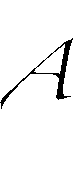
\includegraphics[width=0.3\hsize]{a} 
%   \caption{Figure example}
%   \label{fig:example}
%\end{figure}



%\begin{table}[htbp]
%\caption{Table example }
%\begin{center}
%\begin{tabular}{lcc}
%\toprule
%Title line & xx & yy \\
%\midrule
%l1 &x1  & y1 \\
%l2 &x2  & y2 \\
%\bottomrule
%\end{tabular}
%\end{center}
%\label{tab:example}
%\end{table}%

%In Table\,\ref{tab:example}, the ... \cite{ex}.


%=====================
\chapter{Représentation aléatoire de l'exposant}
\section{State of the art\dots}

Afin d'améliorer l'efficacité de l'exponentiation, il est possible de précalculer certaines valeurs et de changer la représentation
de l'exposant en fonction de ces nombres.
La première partie explicite l'algorithme d'exponention basé sur le précalcul, puis les parties suivantes donnent $3$ méthodes
différentes de représentation.

\subsection{Précalcul et Exponentiation}

Soit $\mathcal{G}$ un groupe et $\mathcal{D}$ un ensemble d'entiers positifs impairs.
Soit $k=(k_{l-1} \ldots k_0)_2$ un entier, où les $k_i$ sont des éléments de $\mathcal{D}$, et soit $g \in \mathcal{G}$.
L'algorithme est en deux étapes :
\begin{itemize}
 \item [1)] Calculer $g^d$, où $d$ sont les éléments de $\mathcal{D}$
 \item [2)] Si $k_i \neq 0$, multiplier par l'élément précalculé $g^{k_i}$
\end{itemize}

\begin{algorithm}
 \caption{Algorithme d'exponentiation avec précalcul}
 \begin{algorithmic}
  \REQUIRE un élément $g$, un entier $N$ positif, un entier $k$ avec $k = (k_{l-1},k_1,\ldots,k_n)$ with $k_i \in \mathcal{D}$
  \ENSURE $g^k \mod N$
  \STATE $S \leftarrow 1$
  \FOR{$i$ from $n$ to $0$}
  \STATE $S \leftarrow S \times S \mod N$
  \IF{$k_i \neq 0$}
  \STATE $S \leftarrow S \times g^{k_i} \mod N$
  \ENDIF
  \ENDFOR
 \end{algorithmic}
\end{algorithm}

A la différence de l'algorithme classique, on multiplie par une valeur $g^{k_i}$ qui dépend de la valeur 
du bit numéro $i$ lorsque celui est non nul (dans l'algorithme classique on a $\mathcal{D} = \{1\}$, et donc 
le seul élément précalculé est $g^1 = g$, c'est donc l'élément que l'on multiplie à chaque bit non nul).

\subsection{Représentation $NAF$ (Non Adjacent Form)}
La représentation $NAF$ est l'unique représentation d'un nombre en entiers relatifs pour laquelle le poids de Hamming est minimal.

\begin{Exemple}
 Le nombre $7$ s'écrit comme :
 $$\begin{array}{ccccccc}
  (0 & 1 & 1 & 1)_2 & = & 4 + 2 + 1 & = 7 \\
  (1 & 0 & -1 & 1)_2 & = & 8 - 2 + 1 & = 7 \\
  (1 & -1 & 1 & 1)_2 & = & 8 - 4 + 2 + 1 & = 7 \\
  (1 & 0 & 0 & -1)_2 & = & 8 - 1 & = 7 \\
 \end{array}$$
 
 La représentation $NAF$ de $7$ est la dernière $$\begin{array}{cccc} (1 & 0 & 0 & -1)_2 \end{array}$$.
\end{Exemple}

\subsection{Représentation $wNAF$ (window Non Adjacent Form)}

L'idée est de recoder l'exposant avec d'autres coefficients que $-1$, $0$ et $1$ en ajoutant tous les nombres 
impairs inférieurs à $2^w$ avec $w$ appelée la taille de la fenêtre.

Soit $\mathcal{B} = \{1,3,\ldots,2^w - 1\}$, la représentation $wNAF$ de $k$ est l'unique représentation 
de $k$ telle que : 
$$\begin{array}{lcccc}
k = & (b_n & \ldots & b_1 & b_0)_2
\end{array}$$ où $b_i \in \mathcal{B} \cup (-\mathcal{B}) \cup \{0\}$, c'est-à-dire $b_i$ peut être égal à 
$0$, un élément de $\mathcal{B}$ ($1$, $3$ , \ldots) ou à l'opposé d'un élément de $\mathcal{B}$ ($-1$, $-3$, \ldots). \\
Et ainsi $k$ vérifie :
\begin{eqnarray*}
 k = \sum_{i=0}^{n} b_i 2^i
\end{eqnarray*}

L'utilité de cette représentation est de réduire le poids de Hamming de la représentation de $k$, 
et de ce fait réduire le temps de calcul de $x^k \mod N$.

\begin{Exemple}
 Le nombre $88$ s'écrit comme :
  $$\begin{array}{cccccccccc}
  (1 & 0 & 1 & 1 & 0 & 0 & 0)_2 & = & 64 + 16 + 8 & = 88 
 \end{array}$$
 
 Pour calculer la représentation $3NAF$ de $88$, il faut définir $\mathcal{B} = \{1,3,5,7\}$.
 En regarder les $3$ premiers bits de poids fort de $88$, on peut remplacer $(101)_2$ par $5$, 
 puis en regardant les $3$ suivants , puis à nouveau les suivants , on remarque qu'on ne peut pas remplacer 
 les coefficients, on obtient donc :
  $$\begin{array}{cccccccc}
  (5 & 1 & 0 & 0 & 0)_2 & = & 5 \times 16 + 8 & = 88 
 \end{array}$$
\end{Exemple}

\subsection{Fractional Windows}

Cette méthode consiste à adapter la taille de $w$ au fil de l'algorithme.
La taille de la fenêtre ($3$ dans l'exemple précédent) n'est plus fixée, elle est adaptée au fil de l'algorithme
afin d'optimiser la vitesse et les calculs de l'algorithme d'exponentiation.


\section{Randomisation et Optimisation}

La partie précédente a présenté les bases et prérequis pour la compréhension de l'article de Nicolas Méloni.
La partie suivante s'intéresse à la méthode d'exponentiation modulaire expliqué dans l'article, 
et à un moyen d'implémenter cette méthode le plus efficacement possible. 
L'idée de la méthode est de recoder de manière aléatoire l'exposant (secret).

Dans la première section, est expliquée la méthode de randomisation détaillée dans son article, puis la deuxième
section détaille l'implémentation de cette méthode et l'optimisation de l'algorithme trouvé, 
finallement la troisième partie correspond à la démonstration de la validité de cet algorithme.

\subsection{Randomisation dans l'algorithme de Fractional Windows}

L'idée de l'algorithme de recodage de l'exposant $k$ est de changer à chaque éxecution de système de codage,
et plus particulièrement de changer l'ensemble des coefficients $\mathcal{D}$.

Soit $k$ l'exposant, $N$ le modulo et $x$ le message.
On pose $\mathcal{D} = \{d_1,\ldots,d_l\}$ où $d_l$ sont des entiers positifs impairs.

Le premier constat révélé dans l'article est que pour pouvoir recoder la totalité des exposants, il faut nécessairement
que $1$ soit dans $\mathcal{D}$.

\subsubsection{La fonction \emph{digit}}

Soit $w > 0$ un entier. Pour tout entier $x$ on définit $p_w(x) = x \mod 2^w $. 
Puis on pose $\mathcal{D}_w = p_w(\mathcal{D})$ et $\overline{\mathcal{D}_w} = \mathcal{D}_w \cup \{2^w - d: d \in \mathcal{D}_w\}$.
Finalement on définit $W_n = \lfloor log_2(max_i(d_i)) \rfloor$.

Pour construire la fonction \emph{digit}, on doit d'abord définir, pour tout k entiers $k$, $w_{max}(k)$ comme le plus grand nombre $w \leq W_n+2$ tel qu'il existe un élément $d_i \in \mathcal{D}$ qui satisfait ces deux conditions :

\begin{itemize}
 \item [1.] $d_i < k$,
 \item [2.] $p_w(k) \in \overline{\mathcal{D}_w}$
\end{itemize}

Finalement, la fonction $digit_{\mathcal{D}}$ : $\mathbb{N} \rightarrow \overline{\mathcal{D}} \cup \{0\}$ est définie par :

\begin{itemize}
 \item [$\bullet$] si $k$ est pair : $digit(k) = 0$,
 \item [$\bullet$] si $k$ est impair :
 \begin{itemize}
  \item [-] on pose $W_{max} = w_{max}(k)$
  \item [-] si $p_{W_{max}}(k) \in \mathcal{D}_{W_{max}}$, $digit_{\mathcal{D}}(k) = d$ avec $d < k$ tel que $p_w(k) = p_w(d)$
  \item [-] si $2^{W_{max}} - p_{W_{max}}(k) \in \mathcal{D}_{W_{max}}$, $digit_{\mathcal{D}}(k) = -d$ avec $d < k$ tel que $2^{W_{max}} - p_w(k) = p_w(d)$
 \end{itemize} 
\end{itemize}

La fonction \emph{digit} est bien définie pour tout $k$ dans $\mathbb{N}$.
De plus, on peut remarquer que $1 \in \mathcal{D}$, ce qui implique que $1 \in \mathcal{D}_w$
pour tout $w$, et donc $W_{max} \geq 2$.

Voici un exemple simple pour bien comprendre la fonction \emph{digit} :
\begin{Exemple}
 On pose $k = 101$ et $\mathcal{D} = \{1,3,9\}$, on a donc $W_n = 3$.
 
 Pour calculer la fonction \emph{digit}, il faut d'abord déterminer $w_{max}(k)$.
 
 On pose $w = W_n + 2 = 5$, on calcule $p_w (k) = 101 \mod 2^5 = 5 \mod 32$. \\
 Puis on calcule $\overline{\mathcal{D}_w} = \{1,3,9,32-1,32-3,32-9\} = \{1,3,9,31,29,23\}$. \\
 On vérifie si $5 \in \overline{\mathcal{D}_w}$, ce n'est pas le cas, donc on pose $w = 4$ et on recommence
 le processus.
 
 On a $p_w (k) = 5 \mod 16$. \\
 Puis on calcule $\overline{\mathcal{D}_w} = \{1,3,9,15,13,7\}$. \\
 On a $5 \notin \overline{\mathcal{D}_w}$, donc on pose $w = 3$.
 
 On a $p_w (k) = 5 \mod 8$. \\
 Puis on calcule $\overline{\mathcal{D}_w} = \{1,3,9 \mod 8,8-1,8-3,8-9 \mod 8\} = \{1,3,5,7\}$. \\
 On a $5 \in \overline{\mathcal{D}_w}$, donc on a $w_{max}(k) = 3$. On pose $W_{max} = w_{max}(k)$.
 
 Ici, on est dans le cas où $k$ est impair, et $2^{W_{max}} - p_{W_{max}} \in \mathcal{D}_{W_{max}}$,
 donc on a $digit_{\mathcal{D}}(k) = -3$ car $2^{W_{max}} - p_w(k) = 2^3 - 5 = 3$.
\end{Exemple}


\subsubsection{L'algorithme de représentation}

Une fois la fonction \emph{digit} définie, l'algorithme de la représentation est le suivant :

\begin{algorithm}
 \caption{Représentation aléatoire de $k$}
 \begin{algorithmic}
  \REQUIRE Un entier $k$ et un ensemble $\mathcal{D} = \{1,d_2,\ldots,d_n\}$
  \ENSURE $k = (k_t k_{t-1} \ldots k_1 k_0)_2$, $k_i \in  \overline{\mathcal{D}} \cup \{0\}$
  \STATE $i \leftarrow 0$
  \WHILE{$k != 0$}
  \STATE $k_i \leftarrow digit_{\mathcal{D}}(k)$
  \STATE $k \leftarrow \frac{k-k_i}{2}$
  \STATE $i \leftarrow i+1$
  \ENDWHILE
  \RETURN $(k_{i-1} \ldots k_0)$
 \end{algorithmic}
\end{algorithm}

\subsubsection{Première implémentation}

Le coeur de l'implémentation de la représentation réside dans celle de la fonction \emph{digit}.
Voici l'algorithme avec lequel j'ai implémenté la fonction \emph{digit} au premier essai : \\
Il est composé de deux parties :
\begin{itemize}
 \item [1)] Un algorithme qui calcule $i$ tel que $p_{W_{max}}(k) = p_{W_{max}}(d_i)$ où $d_i \in \overline{\mathcal{D}}$.
 \item [2)] L'algorithme de la fonction
\end{itemize}

1) L'idée est de partir de la fenêtre de longueur maximale $w=W_n+2$ et de chercher dans $\overline{\mathcal{D}_w}$
si $p_w(k)$ est dedans, s'il n'y est pas on diminue $w$ jusqu'à trouver $p_w(k)$.

\begin{algorithm}
 \caption{Calculer $i$ tel que $p_{W_{max}}(k) = p_{W_{max}}(d_i)$}
 \begin{algorithmic}
  \REQUIRE Un entier $k$, le nombre $W_n$ et un ensemble $\mathcal{D} = \{1,d_2,\ldots,d_n\}$
  \ENSURE $i$ tel que $p_{W_{max}}(k) = p_{W_{max}}(d_i)$ où $d_i \in \overline{\mathcal{D}}$
  \STATE $c = 0$  
  \STATE $w \leftarrow W_n+2$
  \WHILE{$w > 1$ et $c \neq 1$}
  \STATE $\overline{\mathcal{D}_w} \leftarrow p_w(\overline{\mathcal{D}})$
  \STATE $p_k = p_w(k)$
  \STATE $i = 0$
  \WHILE{$c \neq 1$ et $i < 2 \times \#D$}
  \IF{$p_k$ = $\overline{\mathcal{D}_w}[i]$}
  \STATE $c \leftarrow 1$
  \ENDIF
  \STATE $i \leftarrow i+1$
  \ENDWHILE
  \STATE $w \leftarrow w-1$
  \ENDWHILE
  \RETURN $i-1$
 \end{algorithmic}
\end{algorithm}

On conviendra que, d'après l'algorithme, $i$ est nécessairement compris entre $0$ et $2 \#D - 1$

2) A partir de cet algorithme, je peux désormais construire l'algorithme
qui calcule la fonction \emph{digit}.

\begin{algorithm}
 \caption{Calculer $digit_{\mathcal{D}}(k)$}
 \begin{algorithmic}
  \REQUIRE Un entier $k$, le nombre $W_n$ et un ensemble $\mathcal{D} = \{1,d_2,\ldots,d_n\}$
  \ENSURE $digit_{\mathcal{D}}(k)$
  \STATE $digit \leftarrow 0$  
  \IF{$k$ est impair}
  \STATE $i = algorithm4(k,W_n,\mathcal{D})$
  \IF{$i < \#D$}
  \STATE $digit \leftarrow \mathcal{D}[i]$
  \ELSE
  \STATE $digit \leftarrow -\mathcal{D}[i-taille]$
  \ENDIF
  \ENDIF
  \RETURN $digit$
 \end{algorithmic}
\end{algorithm}

\newpage

\subsection{Optimisation de l'algorithme}

L'idée de l'optimisation est de réduire l'appel à la fonction de recherche d'élément dans un tableau dans \emph{Algorithm 4}.
Rechercher dans un tableau ou une table (ou un ensemble) est chronophage en programmation, ainsi pour réduire
le temps et le coût d'éxecution de la représentation, nous avons pensé à un autre algorithme.
Notre idée est basée sur les trois propositions suivantes :
\begin{itemize}
 \item[$\bullet$] Construire un unique tableau d'éléments de $\mathcal{D}$.
 \item[$\bullet$] L'index du tableau correspond à l'antécédant et la case à l'image de l'index.
 \item[$\bullet$] Le remplissage du tableau nécessite uniquement des additions, des multiplications et des modulos.
\end{itemize}

\subsubsection{\emph{Digit} vue comme un tableau}

Afin d'éviter l'appel à une recherche de table, nous avons abordé la fonction \emph{digit} de manière différente,
non pas comme une fonction mais comme la composition d'un modulo et d'une fonction défini par un vecteur.
L'algorithme de la fonction \emph{digit} suit ces étapes :
\begin{itemize}
 \item [1)] Construction d'un tableau \emph{$D_{max}$} de taille $2^{W_n+2}$ où $W_n$ est la taille du plus grand élément de $\mathcal{D}$
 \item [2)] Remplissage de tableau \emph{$D_{max}$} tel que pour $i \in \{0,\ldots,2^{W_n+2}-1\}$, $D_{max}[i] = digit(i)$
 \item [3)] Calcul de $k_{mod} = k$ Mod $2^{W_n+2}$
 \item [4)] Renvoi de $D_{max}[k_{mod}] = digit(k)$
\end{itemize}

\subsubsection{Construction de \emph{$D_{max}$}}

Avant de calculer et de compléter le tableau \emph{$D_{max}$}, il faut calculer $W_n$ et $\overline{\mathcal{D}} = \mathcal{D} \cup (-\mathcal{D})$.

\begin{Construction}
La construction du tableau \emph{$D_{max}$} comporte $3$ principales étapes :
\begin{itemize}
 \item[$\bullet$] Initialiser toutes les cases à $0$ et mettre les éléments de $\overline{D}$ à leur place ($D_{max}[1] = 1$, $D_{max}[23] = 23$).
 \item[$\bullet$] Pour $i$ de $W_n+1$ à $3$, on ajoute $2^i \times (2l+1)$ à chaque élément $\overline{D}$ avec $0 \leq l < 2^{W_n+2-i-1}$ et on complète le tableau avec ces valeurs. 
 \item[$\bullet$] On complète les cases impaires qui valent $0$ avec $1$ ou $-1$ suivant la case.
\end{itemize}

 \begin{algorithm}
  \caption{Calculer $D_{max} = [1,d_i,\ldots,d_i']$ avec $d_i,d_i' \in \overline{\mathcal{D}}$}
  \begin{algorithmic}
   \REQUIRE $W_n$ et $\mathcal{D}$
   \ENSURE $D_{max} = [1,d_i,\ldots,d_i']$ avec $d_i,d_i' \in \overline{\mathcal{D}}$
   \STATE $sizeD \leftarrow |D|$
   \FOR{$k$ de $0$ à $sizeD-1$}
   \STATE $\overline{D}[k] \leftarrow D[k]$
   \STATE $\overline{D}[sizeD+k] \leftarrow 2^{W_n+2}-D[k]$
   \ENDFOR
   \FOR{$k$ de $0$ à $2^{W_n+2}-1$}
   \STATE $D_{max}[k] \leftarrow 0$
   \ENDFOR
   \FOR{$k$ de $0$ à $sizeD-1$}
   \STATE $D_{max}[\overline{D}[k]] \leftarrow D[k]$
   \STATE $D_{max}[\overline{D}[taille+k]] \leftarrow -D[k]$
   \ENDFOR
   \WHILE{$i \geq 3$}
   \STATE $j \leftarrow 2 \times sizeD$
   \STATE $borne \leftarrow 2^{W_n+2-i-1}$
   \WHILE{$j \geq 0$}
   \FOR{$k$ de $0$ à $borne-1$}
   \STATE $d \leftarrow \overline{D}[j] + 2^{i} \times (2k+1)$ Mod$(2^{W_n+2})$
   \IF{$D_{max}[d] = 0$}
   \IF{$j<sizeD$}
   \STATE $D_{max}[d] \leftarrow \overline{D}[j]$
   \ELSE[$j \geq sizeD$]
   \STATE $D_{max}[d] \leftarrow -\overline{D}[j-taille]$
   \ENDIF
   \ENDIF
   \ENDFOR
   \STATE $j \leftarrow j-1$
   \ENDWHILE   
   \STATE $i \leftarrow i-1$
   \ENDWHILE
  \end{algorithmic}
 \end{algorithm}
\end{Construction}

\subsection{Preuve}

Dans cette partie, nous allons montrer que l'algorithme construit à partir de \emph{$D_{max}$} calcule la fonction \emph{digit}

\subsubsection{La fonction \emph{digit} sous forme mathématique}

On peut remarque que calculer la fonction \emph{digit} revient à trouver une fonction vérifiant cette propriété :

\begin{Propriété}
 Soit $\phi_{1_\mathcal{D}} : \mathbb{N} \rightarrow \mathbb{Z} / 2^{W_n+2} \mathbb{Z}$, la projection canonique restreint à $\mathbb{N}$, \\ 
 et $\phi_{2_\mathcal{D}} : \mathbb{Z} / 2^{W_n+2} \mathbb{Z} \rightarrow \overline{\mathcal{D}} \cup \{0\}$ une fonction.
 
 On a $digit_{\mathcal{D}} = \phi_{2_\mathcal{D}} \circ \phi_{1_\mathcal{D}}$ $\iff$
 $\forall k$, $\bar{k} = \phi_1(k) = k$ Mod $2^{W_n+2}$ et : \\
 \begin{itemize}
  \item [(i)] Si $k$ est pair $\phi_{2_\mathcal{D}}(\bar{k}) = 0$
  \item [(ii)] Si $k$ est impair $\phi_{2_\mathcal{D}}(\bar{k}) = d_i$, avec $d_i \in \overline{\mathcal{D}} 
  \Rightarrow \exists j \in \llbracket 2,W_n+2 \rrbracket$,
 tel que $k = d_i$ Mod $2^j$ et $\forall m \in \llbracket j+1,W_n+2 \rrbracket, \forall d'_i \in \overline{\mathcal{D}}, k \neq d'_i$ Mod $2^m$.
 \end{itemize}
\end{Propriété}

\begin{Remarque}
 La condition (ii) explique que le $j$ que l'on trouve doit être le plus grand possible. 
\end{Remarque}

\begin{Preuve}
 On prouve la double implication pour tout $k$ dans $\mathbb{N}$.
 
 D'abord si $k$ est pair, c'est évident car les deux fonctions valent $0$ et $\phi_{1_\mathcal{D}}(k)$ est ``paire'' pour $k$ pair et ne peut valoir $0$ si $k$ est impair.
 
 Maintenant si $k$ est impair. Commençons avec l'implication $\Leftarrow$ :
 \begin{itemize}
  \item [$\Leftarrow$] Soit $\phi_{2_\mathcal{D}}$ verifiant les conditions (i) and (ii). \\
  Alors $\exists j \in \llbracket 2,W_n+2 \rrbracket$,
 tel que $k = d_i$ Mod $2^j$ et $\forall m \in \llbracket j+1,W_n+2 \rrbracket, \\
 \forall d'_i \in \overline{\mathcal{D}}, \bar{k} \neq d'_i$ Mod $2^m$. \\
 So $\forall m > j$, $p_m(k) \notin \overline{\mathcal{D}_m}$. \\
 That implies $w_{max} \leq j$. \\
 Furthermore $\bar{k} = d_i$ Mod $2^j$ with $d_i$ in $\overline{\mathcal{D}}$, which means $p_j(k) \in \overline{\mathcal{D}}_j$.
 Finally we have $w_{max} = j$.
  \begin{itemize}
   \item [$\bullet$] Si $d_i \in \mathcal{D}$,  $p_j(k)=p_j(d_i) \Rightarrow digit_{\mathcal{D}}(k) = \phi_{2_\mathcal{D}}(\bar{k})$.
   \item [$\bullet$] Si $-d_i \in \mathcal{D}$, $p_j(k)=p_j(d_i) \Rightarrow 2^j - p_j(k)=p_j(-d_i) \Rightarrow 2^j - p_j(k) \in \mathcal{D}$. \\
   And so $digit_{\mathcal{D}}(k) =-(-d_i)=d_i=\phi_{2_\mathcal{D}}(\bar{k})$.
  \end{itemize}
  \item [$\Rightarrow$] On suppose que l'on a $digit_{\mathcal{D}}(k) = \phi_{2_\mathcal{D}}(\bar{k}) = d_i$ ou $-d_i$ avec $d_i \in \mathcal{D}$. \\
  On a $digit_{\mathcal{D}}(k) = d_i$ avec $d_i \in \overline{\mathcal{D}_m}$. \\
  Let $j = w_{max}(k) = W_max$. \\
  Par definition de $w_{max}(k)$, la condition $2)$ est fausse $\forall m > j$, 
  donc $\nexists d'_i \in \mathcal{D}$ tel que $p_m(k) \in \overline{\mathcal{D}_m}$. \\
  Ainsi $\forall m > j$, $\forall d'_i \in \overline{\mathcal{D}}$, $k \neq d'_i$ Mod $2^m$.
  
  De plus $j=w_{max} \Rightarrow w_{max}$ satisfait la condition $2)$, \\
  i.e. $p_j(k) \in \overline{\mathcal{D}_j} \Rightarrow \exists d_i \in \overline{\mathcal{D}}$ tel que $k = d_i$ Mod $2^j$.
 \end{itemize}

\end{Preuve}

\subsubsection{Preuve de fonctionnement de \emph{$D_{max}$}}

\begin{Proposition}
 Soit $\phi_{1_\mathcal{D}} : \mathbb{N} \rightarrow \mathbb{Z} / 2^{W_n+2} \mathbb{Z}$ la projection canonique restreint à $\mathbb{N}$
 et $\phi_{2_\mathcal{D}} : \mathbb{Z} / 2^{W_n+2} \mathbb{Z} \rightarrow \overline{\mathcal{D}} \cup \{0\}$ tel que $\phi_{2_\mathcal{D}}(\bar{k}) = D_{max}[\bar{k}]$.
 Donc on a $digit_{\mathcal{D}} = \phi_{2_\mathcal{D}} \circ \phi_{1_\mathcal{D}}$.
\end{Proposition}

\begin{Preuve}
 Par construction $\phi_{2_\mathcal{D}} : \mathbb{Z} / 2^{W_n+2} \mathbb{Z} \rightarrow \overline{\mathcal{D}} \cup \{0\}$ donc $\phi_{2_\mathcal{D}}$ existe.
 Par la propriété $1$, on doit prouver que $\phi_{2_\mathcal{D}}$ vérifie $\forall k$ : \\
 \begin{itemize}
  \item [(i)] Si $k$ est pair $\phi_{2_\mathcal{D}}(\bar{k}) = 0$
  \item [(ii)] Si $k$ est impaire $\phi_{2_\mathcal{D}}(\bar{k}) = d_i$, avec $d_i \in \overline{\mathcal{D}} 
  \Rightarrow \exists j \in \llbracket 2,W_n+2 \rrbracket$,
 tel que $k = d_i$ Mod $2^j$ et $\forall m \in \llbracket j+1,W_n+2 \rrbracket, \forall d'_i \in \overline{\mathcal{D}}, k \neq d'_i$ Mod $2^m$.
 \end{itemize}
 
 Maintenant regardons la preuve :
 \begin{itemize}
  \item [(i)] La première condition est vérifiée parce que $D_{max}[l] = 0$ pour $0 \leq l < 2^{W_n+2}$ (initialisation) et le tableau est complété en ajoutant des éléments impairs (les impairs de $\mathcal{D}$ et $d+2p$, $d$ dans $\mathcal{D}$).
  \item [(ii)] La deuxième condition est plus difficile à prouver.
  
  Par construction $\phi_{2_\mathcal{D}}(\bar{k}) = d_i$ avec $d_i \in \overline{\mathcal{D}}$ signifie
  $\exists j \in \llbracket 2,W_n+2 \rrbracket$ s.t. $\bar{k} = d_i + (2l+1)2^j$ Mod $2^{W_{max}}$ avec $0 \leq l < 2^{W_n+2-j-1}$, (1) \\
  et $\forall m > j$, $\nexists d'_i, l'$ tel que $\bar{k} = d'_i + (2l'+1)2^m$ Mod $2^{W_n+2}$. (1bis) \\
 \end{itemize}
  \vspace{0.3cm}
  
  La relation (1) implique $\exists j$ tel que $k = \bar{k} = d_i$ Mod $2^j$. \\
  Maintenant il faut montrer que $\forall m \in \llbracket j+1,W_n+2 \rrbracket, \forall d'_i \in \overline{\mathcal{D}}, k \neq d'_i$ Mod $2^m$. \\
  Par l'absurde on suppose qu'il existe un tel $m > j$ et $d'_i \in \overline{\mathcal{D}}$ tel que :
  \begin{center} $k = d'_i$ Mod $2^m$. (2) \end{center}
  By (2), on a $k = d'_i + n \times 2^m$ Mod $2^{W_n+2}$ avec $0 \leq n < 2^{W_n+2-m}$. (3) \\
  Par distinction de cas, on a :
  \begin{itemize}
   \item[$\bullet$] Si $n = 0$, (3) $\Rightarrow$ $k = d'_i$ Mod $2^{W_n+2}$, contradiction avec la construction de $D_{max}$ (on complète d'abord le tableau avec les éléments de $\overline{\mathcal{D}}$).
   \item[$\bullet$] Si $n$ est pair, i.e. $n = 2n'$, soit $m'=m+1$ et \\
   (3) $\Rightarrow k = d'_i + n' \times 2^{m'}$ Mod $2^{W_n+2}$. Si $n'$ est encore pair, on réitère le procédé jusqu'à ce que $n'$ soit pair.
   On réduit le problème au cas $n$ impair.
   \item[$\bullet$] Si $n$ est impair, i.e. $n = 2l'+1$. \\
   Alors (3) $\Rightarrow k = d'_i + (2l'+1) \times 2^m$ Mod $2^{W_n+2}$ avec $0 \leq 2l'+1 < 2^{W_n+2-m}$. \\
   Et $0 \leq 2l'+1 < 2^{W_n+2-m} \Rightarrow 0 \leq l' < 2^{W_n+2-m-1}$. \\
   Finalement on a $k = d'_i + (2l'+1) \times 2^m$ Mod $2^{W_n+2}$ avec $0 \leq l' < 2^{W_n+2-m-1}$.
   Il y a contradiction avec (1bis). Impossible.
   \end{itemize}
  
  Donc $\phi_{2_\mathcal{D}}$ vérifie la seconde condition and d'après la propriété,
 on a $digit_{\mathcal{D}} = \phi_{2_\mathcal{D}} \circ \phi_{1_\mathcal{D}}$.
\end{Preuve}

\begin{Corollaire}
 On peut utiliser l'algorithme de construction de \emph{$D_{max}$} pour calculer la fonction \emph{digit}.
\end{Corollaire}

\subsection{Test et Performance}

Nous avons effectuer des tests de performance afin de déterminer l'influence de cette méthode de randomisation de la représentation sur la vitesse d'exponentiation.

\subsubsection{Comparaison avec $wNAF$}

\begin{table}[htbp]
\caption{Temps d'execution (10000 tests) }
\begin{center}
\begin{tabular}{ccccc}
\toprule
\#D & |k| & $RDR$ & $wNAF$ & perte (en \%) \\
\midrule
4 & 256 & 373  & 244 & 54\\
4 & 4096 & 11950 & 10820 & 10 \\
8 & 256 & 342 & 224 & 52 \\
16 & 4096 & 12101 & 10585 & 14 \\
32 & 256 & 526 & 214 & 146 \\
64 & 256 & 1108 & 220 & 504 \\
64 & 4096 & 12481 & 10538 & 18 \\
\bottomrule
\end{tabular}
\end{center}
\label{tab:example}
\end{table}%

In Table\,\ref{tab:example}, the ... \cite{ex}.

On remarque que pour plus la taille de $k$ augmente, plus la perte relative diminue.
Cependant pour une taille plus petite de $k$ petite ($256$ bits), la perte est significative ($> 50 \%$),
et plus particulièrement lorsqu'on augmente la taille de $\mathcal{D}$.

\chapter{Etat de l'art de la double exponentiation}

La partie précédente a permis de comprendre la $RDR$ (Random Digit Representation) proposée par Nicolas Méloni.
Cette partie s'intéresse à la généralisation de la $RDR$ pour la multi-exponentiation et plus particulièrement
pour la double exponentiation, c'est-à-dire au calcul de $g^a \times h^b$, où $g$ et $h$ sont des 
éléments de $\mathcal{G}$ (un groupe), et $a$ et $b$ des entiers naturels.

Le procédé de multi-exponentiation est très utilisé dans les protocoles de signatures, que ce soit à base 
de courbes elliptiques, ou dans d'autres cas comme dans la signature El-Gamal.

Pour se faire, il est important de rappeler l'état de l'art de la double exponentiation. \\
La première partie explique l'approche de Shamir dans la double exponentiation. \\
La seconde partie donne la méthode qui a servi de base pour construire la $DoubleRDR$ 
(la $RDR$ étendue à la double exponentiation).

\section{L'approche de Shamir}

Dans un premier temps, je donne la méthode naïve de la double exponentiation afin de constater comment Shamir
a réussi à l'optimiser dans les parties suivantes.

\subsection{La méthode naïve}

La méthode la plus simple pour calculer $g^a \times h^b$ est de calculer $g^a$ et $h^b$ séparement, puis de les multiplier
entre eux.

Appliquer ce processus revient à effectuer deux exponentiations et une multiplication, ce qui fait en moyenne
$2l$ ``square'' et $l$ multiplications, où $l$ est la taille de $a$ et de $b$ (approximativement).

\subsection{Le ``square'' en simultané}

Le premier constat de Shamir fut qu'il était possible de faire un ``square'' pour les deux exposants à la fois.

Pour illustrer cette méthode, je prend l'exemple suivant :

Soit $a=37$ et $b=20$, ie on cherche à calculer $g^{37} h^{20}$.

  $$\begin{array}{cccccccc}
  37 = & (1 & 0 & 0 & 1 & 0 & 1) \\
  20 = & (0 & 1 & 0 & 1 & 0 & 0) \\
  \Box       & 1  & g^2   & g^4 h^2 & g^8 h^4 & g^{18} h^{10} & g^{36} h^{20} \\
  \times g & g  & \,    & \,      & g^9 h^4 & \,            & g^{37} h^{20} \\
  \times h & \, & g^2 h & \,      & g^9 h^5 & \,            & \,
 \end{array}$$ 
 
 Le symbole $\Box$ correspond à l'opération ``square'' qu'on effectue à chaque bit. \\
 Les autres symboles $\times g$ et $\times h$ correspondent tout simplement à la multiplication par $g$ et $h$ 
 respectivement.
 
 On s'aperçoit donc que chaque coefficient non nul dans la représentation de $g$ et dans celle de $h$, donne lieu
 à une multiplication, cependant cette technique permet de diviser par $2$ le nombre de ``square'' 
 (seulement $5$ au lieu de $10$ dans notre cas).
 
 Ainsi cette technique donne en moyenne $l$ ``square'' et $l$ multiplications et est appelée
 \emph{Simple Shamir Method}.
 
 
\subsection{Le précalcul}

Le deuxième constat de Shamir concerna les mutliplications, et particulièrement la quatrième colonne du tableau
précédent. Il s'aperçut qu'il était possible d'économiser une multiplication à chaque fois que le coefficient de chaque
exposant était non nul simultanément (comme au bit $4$ pour $37$ et $20$).

Le moyen simple d'éviter ces deux multiplications est de précalculer le produit $g \times h$, et ainsi de 
multiplier directement par $g \times h$ pour économiser une opération à chaque apparition de $1$ sur la même colonne.

Avec le même exemple que dans la partie précédente, on a :

  $$\begin{array}{cccccccc}
  37 = & (1 & 0 & 0 & 1 & 0 & 1) \\
  20 = & (0 & 1 & 0 & 1 & 0 & 0) \\
  \Box       & 1  & g^2 & g^4 h^2 & g^8 h^4 & g^{18} h^{10} & g^{36} h^{20} \\
  \times g & g  & \,    &    \,   &    \,   & \,            & g^{37} h^{20} \\
  \times h & \, & g^2 h &    \,   &    \,   & \,            & \, \\
  \times gh & \, & \,   &    \,   & g^9 h^5 & \,            & \,
  \end{array}$$

 Ainsi cette technique donne en moyenne $l$ ``square'' et $\frac{3l}{4}$ multiplications et est appelée
 \emph{Fast Shamir Method}.

\section{L'approche de Solinas et la $JSF$}

L'approche de Shamir a l'avantage de fonctionner pour tous les groupes, et en particulier dans le cas des courbes 
elliptiques, ainsi il est possible d'utiliser les astuces des parties précédentes dans ce cas.

C'est avec cette idée que Solinas a pensé une méthode pour recoder les deux exposants dans la double exponentiation 
afin d'en accélérer l'execution.

\subsection{Basé sur un $NAF$}

Dans le cas des courbes elliptiques, où le calcul de $-P$ est négligeable comparé à l'addition de points
(analogie entre multiplication scalaire pour les courbes elliptiques et exponentiation modulaire),
on peut utiliser une représentation signée (``signed binary expansion''), c'est-à-dire utiliser $0$, $1$ ET $-1$.

Cependant, étant donné qu'il existe une infinité de représentation signée, on utilise la représentation optimale
(au vu du nombre de $0$) de l'exposant, appelée aussi représentation $NAF$ (vu dans la première partie) qui 
vérifie certaines propriétés.

Solinas est allé encore plus loin en constatant qu'il était encore plus optimal de choisir entre la représentation classique 
et la représentation $NAF$ pour chacun des exposants afin que les coefficients non nuls de chaque recodage se situent
sur les mêmes bits (à la même colonne dans la représentation).

Par exemple, avec les exposants $11$ et $20$, le calcul de $11P + 20Q$ donne :

  $$\begin{array}{ccccccc}
  11 = & (1 & 0 & -1 & 0 & -1) \\
  20 = & (1 & 0 & 1 & 0 & 0) \\
  \times 2 & \mathcal{O} & 2P + 2Q & 4P + 4Q & 6P + 10Q & 12P + 20Q \\
  \pm P      & P           & \,      & 3P + 4Q &    \,    & 11P + 20Q \\
  \pm Q      & P + Q       & \,      & 3P + 5Q &    \,    & \,
  \end{array}$$

  Pour le premier exposant, j'ai opté pour la représentation $NAF$ alors que pour le deuxième exposant, j'ai choisi la représentation classique.
  Le résultat est que le nombre de zéros sur la même colonne permet d'économiser des multiplications.
  
  Cette représentation est appelée ``Joint Signed Binary Expansion'', elle est adaptée à la ``Simple Shamir Method'' dans l'exemple.
  Il existe également une adaptation de ce raisonnement avec la ``Fast Shamir Method'' mais elle n'est pas triviale.
  
  Quoiqu'il en soit, la ``Joint Signed Binary Expansion'' nécessite en moyenne $l$ doublages (équivalent du ``square'')
  et $\frac{2l}{3}$ additions avec l'adaption simple, et $l$ doublages et $\frac{5l}{9}$ additions avec l'adaption rapide de Shamir.
  
  C'est avec cette approche que Solinas a trouvé une autre méthode de recodage.

\subsection{La Joint Spar Form}

Dans cette partie, j'expliquerai la méthode de Solinas pour recodant les deux exposants dans la double exponentiation.

Dans un premier temps, j'explicite la notion de poids ``joint'' de Hamming, puis dans un exemple je montre l'avantage de la
$JSF$ sur la représentation $NAF$. Ensuite je donne un exemple concret dont je me servirai dans les prochaines parties,
puis finalement je donne les résultats qu'a obtenu Solinas avec cette méthode.

\subsubsection{Joint Hamming Weight}

Le Poids de Hamming Joint est le nombre de colonnes non nuls dans la représentation de deux nombres.
Une colonne non nul est un bit pour lequel l'un des deux (ou les deux !) exposant(s) a un coefficient non nul.
Par exemple, dans le cas de la partie précèdente, on a :

  $$\begin{array}{ccccccc}
  11 = & (1 & 0 & -1 & 0 & -1) \\
  20 = & (1 & 0 & 1 & 0 & 0)
  \end{array}$$

Le poids de Hamming Joint de cette représentation est $3$ car il y a $3$ colonnes non nuls (et $2$ colonnes $\doublezero$).

Si on applique la Fast Shamir Method à cette représentation, le nombre d'addition est exactement poids de Hamming Joint
de la représentation.

\subsubsection{Comparaison avec $NAF$}

Avant de comprendre la construction de la représentation $JSF$, je montre dans un exemple comparatif l'efficacité
de cette dernière.

Alors que $NAF$ a pour but de minimiser le poids de Hamming de chacun des exposants, la $JSF$ a pour but de
minimiser le Poids de Hamming Joint.

Dans l'exemple ci-dessous, on remarque qu'avec la représentation $NAF$ :

  $$\begin{array}{cccccccccc}
  53 = & (0 & 1 & 0 & -1 & 0 & 1 & 0 & 1) \\
  102 = & (1 & 0 & -1 & 0 & 1 & 0 & -1 & 0)
  \end{array}$$

  Le poids de Hamming Joint est $8$ (il n'y a aucun $\doublezero$).
  
Les mêmes exposants avec la représentation $JSF$ :

  $$\begin{array}{cccccccccc}
  53 = & (0 & 1 & 0 & 0 & -1 & 0 & -1 & -1) \\
  102 = & (1 & 0 & 0 & -1 & -1 & 0 & -1 & 0)
  \end{array}$$

  Le poids de Hamming Joint est seulement $6$ (il y a $2$ $\doublezero$).
  
  La $JSF$ dans ce cas permet d'économiser deux additions, cependant il faut précalculer $P+Q$ et $P-Q$.
  
\subsubsection{Un exemple simple}

Voici un exemple simple de la Fast Shamir Method appliquée à la $JSF$, avec $53$ et $102$ comme exposants :

  $$\begin{array}{cccccccccc}
  53  = & (0 & 1 & 0 &  0 & -1 & 0 & -1 & -1) \\
  102 = & (1 & 0 & 0 & -1 & -1 & 0 & -1 &  0) \\
  \times 2   & \mathcal{O} & 2Q   & 2P+4Q & 4P+8Q & 8P+14Q & 14P+26Q & 28P+52Q & 54P+102Q \\
  \pm P      &             & P+2Q & \,    & \,    & \,     & \,      & \,      & 53P+102Q \\
  \pm Q      & Q           & \,   & \,    & 4P+7Q & \,     & \,      & \,      & \,       \\
  \pm (P+Q)  &             & \,   & \,    & \,    & 7P+13Q & \,      & 27P+51Q & \,       \\
  \pm (P-Q)  &             & \,   & \,    & \,    & \,     & \,      & \,      & \,
  \end{array}$$
  
  Cette méthode nécessite en moyenne $l$ doublages et $\frac{l}{2}$ additions.
  
\chapter{Approche du problème}

La partie précédente a rappelé l'état de l'art de la double exponentiation, cette partie s'intéresse à la 
problèmatique suivante : peut-on étendre la $RDR$ de Nicolas Méloni à la double exponentiation ?

L'objectif principal de la $RDR$ est la protection de l'algorithme d'exponentiation contre les attaques 
par canal auxiliaire. Ainsi, la $DoubleRDR$ ($RDR$ étendue à la double exponentiation) doit pouvoir utiliser des
coefficients quelconques (impairs). Il faut également que les résultats ne dépendent pas des coefficients 
choisis sous peine de voir la méthode vulnérable à une attaque ``side channel''.

L'objectif secondaire de la $DoubleRDR$ est de rendre l'exponentiation modulaire la plus efficace possible.

Dans une première section, on définit la $DoubleRDR$ et les contraintes associées.

La deuxième section détaille la méthode générale de la $DoubleRDR$.

Puis la dernière section donne un exemple de $DoubleRDR$ de deux exposants afin de mieux comprendre la méthode.

\section{La représentation d'un couple d'exposants}

Dans cette partie, on fixe un couple d'exposants $(k_1,k_2) = (53,102)$ et un ensemble $\mathcal{D} = \{1,3,23,27\}$,
puis on détermine la représentation idéale, au sens des objectifs fixés, de ce couple.

Solinas a adapté la méthode $NAF$ à la double exponentiation, ainsi il semble possible d'adapter la $RDR$
à la double exponentiation, en utilisant le même procédé.

A l'aide d'un exemple simple, cette partie définit la $DoubleRDR$ au sens des objectifs fixés et des avantages
de cette représentation.

%J'ai essayé d'obtenir un maximum de $\doublezero$ ($JSF$ de Solinas), tout en utilisant les recodages que j'avais 
%déjà à disposition (les $RDR$ pour chacun des exposants), et pour assembler les deux avantages de chaque représentation,
%je me suis inspiré du travail de Solinas qui a adapté la méthode $NAF$ (avec les coefficients $0$ et $\pm 1$) à la double exponentiation.

\subsection{Une solution simple à l'objectif $1$}

Le premier objectif de la $DoubleRDR$ est le recodage des deux exposants à l'aide de coefficients aléatoire
(de cette façon, la $DoubleRDR$ rend l'algorithme d'exponentiation résistant à une attaque ``side-channel'').

Une première approche triviale consiste à utiliser la $RDR$ sur chacun des exposants, de cette manière 
la représentation obtenue utilise les coefficients de $\mathcal{D}$ et remplit l'objectif $1$.

En suivant la $RDR$, on obtient : \\
  $$\begin{array}{cccccccccc}
  53 & = & (1 & 0 & 0 & -3 & 0 & 0 & 0 & -27) \\
  102 & = & (0 & 0 & 3 & 0 & 0 & 0 & 3 & 0)
 \end{array}$$

 Le poids de Hamming Joint de cette représentation est $5$ car il y a trois $\doublezero$ sur huit bits.
 
 Il s'agit de déterminer si cette représentation est la meilleure représentation possible au vu de l'objectif $2$.
 Pour se faire, d'après l'approche de Shamir (Fast Shamir Method), la représentation la plus efficace de $(k_1,k_2)$
 est celle ayant un poids de Hamming Joint minimal, c'est-à-dire un nombre de $\doublezero$ maximal.

\subsection{La $JSF$, solution à l'objectif $2$}

Afin de déterminer la représentation $DoubleRDR$, une seconde approche consiste à utiliser la méthode $JSF$,
méthode la plus efficace pour l'objectif $2$, puis à l'adapter avec des coefficients de $\mathcal{D}$.

Par exemple, la $JSF$ de $(k_1,k_2)$ est : \\
  $$\begin{array}{cccccccccc}
  53 & = & (0 & 1 & 0 & 0 & -1 & 0 & -1 & -1) \\
  102 & = & (1 & 0 & 0 & -1 & -1 & 0 & -1 & 0)
 \end{array}$$
 
 Le poids de Hamming Joint de la représentation est $6$, cependant l'ensemble $\mathcal{D}$ est réduit
 à $\{1\}$. Il est évident que cette représentation présente des avantages en terme d'efficacité, et donc
 des avantages au vu de l'objectif $2$, cependant elle ne remplit pas la condition de l'objectif $1$ car elle
 n'utilise que les coefficients $0$, $1$ et $-1$.
 
 \vspace{1cm}
  
  Ce qui est important dans la méthode $JSF$ est de faire correspondre les coefficients non nuls afin 
 de créer des doubles zéros, comme on peut le voir dans l'exemple ci-dessous :

 Représentation $NAF$ de $53$ et de $102$ :
 
  $$\begin{array}{cccccccccc}
  53 = & (0 & 1 & 0 & -1 & 0 & 1 & 0 & 1) \\
  102 = & (1 & 0 & -1 & 0 & 1 & 0 & -1 & 0)
  \end{array}$$
  
  Représentation $JSF$ de $53$ et de $102$ :

  $$\begin{array}{cccccccccc}
  53 = & (0 & 1 & 0 & 0 & -1 & 0 & -1 & -1) \\
  102 = & (1 & 0 & 0 & -1 & -1 & 0 & -1 & 0)
  \end{array}$$

  Les coefficients non nuls de la première représentation sont tous décalés (il n'y a aucun $0$ sur la même
  colonne, et donc sur le même bit), alors que la deuxième représentation offre l'avantage d'avoir deux $0$
  sur le même bit (c'est-à-dire deux $\doublezero$) et donc un poids de Hamming de $6$ au lieu de $8$.
 
 \subsection{La représentation $DoubleRDR$}

 Voici deux autres représentations possible de $(53,102)$ basées sur les deux premiers recodages $RDR$ et $JSF$ :
 
   $$\begin{array}{cccccccccc}
  53 & = & (1 & 0 & -1 & 0 & 0 & 0 & -23 & 3) \\
  102 & = & (1 & 0 & -1 & 0 & 0 & 0 & 3 & 0)
 \end{array}$$

  Le poids de Hamming Joint de cette représentation est de $4$.
 
Et :
  $$\begin{array}{cccccccccc}
  53 & = & (0 & 0 & 1 & 0 & 0 & 0 & -1 & 23) \\
  102 & = & (0 & 0 & 3 & 0 & 0 & 0 & 3 & 0)
 \end{array}$$
 
 Le poids de Hamming Joint de cette représentation est de $3$.
 
 \vspace{0.5cm}
 
 Voici les premiers constats que l'on peut faire en observant ces résultats : 
 \begin{itemize}
  \item [$\bullet$] La $RDR$ de chacun des exposants $k_1$ et $k_2$ n'est pas la meilleure représentation de
  $(k_1,k_2)$ au sens des objectifs donnés.
  \item [$\bullet$] Une représentation où les coefficients non nuls de chacun des exposants sont à la même place 
  ($1$ et $3$, puis $-1$ et $3$ sur la même colonne) est plus efficace.
 \end{itemize}

De ces constats, on peut définir la $DoubleRDR$ selon les deux objectifs suivants :
\begin{itemize}
 \item [Objectif $1$:] Les coefficients non nuls d'un exposant doivent se situer sur les mêmes bits 
 que les coefficients non nuls de l'autre exposant.
 \item [Objectif $2$:] La représentation doit contenir un maximum de $\doublezero$ consécutifs.
\end{itemize}

\section{Exemple et Contraintes}

\subsection{Exemple}

Prenons un exemple simple afin de comprendre les tenants et les aboutissants de cette méthode.

J'ai choisi $k_1 = 869027$ et $k_2 = 706440$, et $\mathcal{D} = \{1,3,23,27\}$. \\
On a donc $W_{max} = 6$ et $\dbarre = \{1,3,23,27,37,41,61,63\}$.

$$\begin{array}{cccccccccccccccccccccc}
  869027 & = & (1 & 1 & 0 & 0 & 0 & 1 & 0 & 1 & 0 & 1 & 0 & 0 & 0 & 0 & 1 & 0 & 1 & 0 & 1 & 1) \\
  706440 & = & (0 & 0 & 0 & 1 & 0 & 0 & 0 & 1 & 1 & 1 & 1 & 0 & 0 & 0 & 1 & 1 & 0 & 1 & 0 & 1)
 \end{array}$$
 
 Nombre de $\doublezero$ : $6$.

 En appliquant la $RDR$ sur chacun des nombres, on obtient :
 
 $$\begin{array}{ccccccccccccccccccccccc}
  869027 & = & (3 & 0 & 0 & 0 & 0 & -27 & 0 & 0 & 0 & 3 & 0 & 0 & 0 & 0 & -27 & 0 & 0 & 0 & 1 & 0 & 1) \\
  706440 & = & (0 & 0 & 0 & 1 & 0 & 0 & 0 & -1 & 0 & 0 & 0 & -23 & 0 & 0 & 0 & 23 & 0 & 0 & 0 & 0 & 0)
 \end{array}$$

 Nombre de $\doublezero$ : $11$.
 
Maintenant appliquons la méthode sur ces deux exposants, en tout premier lieu il s'agit d'observer les bits faibles de chacun 
des exposants. \\
On a donc $B_{f,1} = 0$ et $B_{f,2} = 3$, et donc $B_{f,1} < B_{f,2}$. \\
Ensuite, comme $B_{f,1} - B_{f,2} = 3$, il s'agit de trouver les coefficients $d_0$ et $d_1$ de $\dbarre$ tels que

  $$\begin{array}{ccc}
k_1 & = & d_0 + 2^3 \times d_1[64] \\
 \end{array}$$

 Pour se faire, on calcule donc $k_1 - \dbarre$.
 Ici $k_1 = 35 [64]$, et donc on a : \\
 $k_1 - \dbarre = \{34,32,12,8,36,38,58,62\}$. \\
 On remarque que $8$ divise $8$, et donc $d_0 = 27$. \\
 Maintenant, il faut vérifier qu'il existe $d_1 \in \dbarre$, pour lequel
 $8 \times d_1 = 8$, ce qui est le cas pour $d_1 = 1$.
 
 Donc on a :
 
 $$\begin{array}{cccccc}
  869027 & = & (27 & 0 & 0 & \ldots \\
  706440 & = & (0 & 0 & 0 & \ldots
 \end{array}$$
 
 Et on effectue :
 $$\begin{array}{cccccc}
  \frac{869027 - 27}{8} & = & 108625 \\
  \frac{706440}{8} & = & 88305
 \end{array}$$
 
Puis on note les bits faibles de chacun des exposants, $B_{f,1} = B_{f,2} = 0$. \\
Comme les bits faibles sont identiques, on calcule $k_1 - \dbarre$ et $k_2 - \dbarre$. \\
Ici $k_1 = 17 [64]$ et $k_2 = 49 [64]$. \\
Ainsi  $k_1 - \dbarre = \{16,14,58,54,18,20,40,44\}$. \\
Et  $k_2 - \dbarre = \{48,46,26,22,50,52,8,12\}$. \\ 
La plus grande puissance de $2$ qui divise un des élément dans chacun des ensembles est $16$
car il y a $16$ dans le premier ensemble et $48$ dans le second. \\
Ainsi pour $d_0 = 1$ pour $k_1$ et $d_0' = 1$ pour $k_2$, il reste à vérifier qu'il existe $d_1$ et 
$d_1'$ tels que :

   $$\begin{array}{ccc}
k_1 & = & 1 + 16 \times d_1[64] \\
k_2 & = & 1 + 16 \times d_1'[64]
 \end{array}$$
 
Ce qui est le cas pour $d_1 = 1$ et $d_1' = 3$. 

Donc on a :
 
 $$\begin{array}{cccccccccc}
  869027 & = & (27 & 0 & 0 & 1 & 0 & 0 & 0 & \ldots \\
  706440 & = & (0 & 0 & 0 & 1 & 0 & 0 & 0 & \ldots
 \end{array}$$
 
 Et on effectue :
 $$\begin{array}{cccccc}
  \frac{108625 - 1}{16} & = & 6789 \\
  \frac{88305-1}{16} & = & 5519
 \end{array}$$
 
 On continue la méthode, on se retrouver dans la même situation que précédemment.
 
 Ainsi on réitère le processus : \\
 Ici $k_1 = 5 [64]$ et $k_2 = 15 [64]$. \\
Ainsi  $k_1 - \dbarre = \{4,2,46,42,6,8,28,32\}$. \\
Et  $k_2 - \dbarre = \{14,12,56,52,16,18,38,42\}$. \\ 
 Cette fois-ci, on remarque que $32$ divise un élément de $k_1 - \dbarre$ mais aucun élément de $k_2 - \dbarre$,
et $16$ divise un élement de $k_2 - \dbarre$ et $32$ pour $k_1 - \dbarre$, cependant comme il a été dit précédemment
il est impossible de trouver un élément $d_1$ tel que $k_1 - d_0 = 32 = 16 \times d_1 [64]$, car dans ce case
on aurait $d_1$ pair et non nul, impossible.

Donc on a $8$ la plus grande puissance de $2$ divisant à la fois un élément de $k_1 - \dbarre$
et un de $k_2 - \dbarre$, et telle que la puissance supérieure ($16$) ne divise pas ces éléments. \\
On prend $d_0 = -3$ pour $k_1$ et $d_0' = 23$ pour $k_2$, il reste à vérifier qu'il existe $d_1$ et 
$d_1'$ tels que :

   $$\begin{array}{ccc}
k_1 & = & -3 + 8 \times d_1[64] \\
k_2 & = & 23 + 8 \times d_1'[64]
 \end{array}$$
 
Ce qui est le cas pour $d_1 = 1$ et $d_1' = -1$.

Donc on a :
 
 $$\begin{array}{ccccccccccccc}
  869027 & = & (27 & 0 & 0 & 1 & 0 & 0 & 0 & -3 & 0 & 0 & \ldots \\
  706440 & = & (0 & 0 & 0 & 1 & 0 & 0 & 0 & 23 & 0 & 0 & \ldots
 \end{array}$$
 
 Et on effectue :
 $$\begin{array}{cccccc}
  \frac{6789 + 3}{8} & = & 849 \\
  \frac{5519-23}{8} & = & 687
 \end{array}$$
 
 On continue la méthode, on se retrouver dans la même situation que précédemment.
 
 Ainsi on réitère le processus : \\
 Ici $k_1 = 17 [64]$ et $k_2 = 47 [64]$. \\
Ainsi  $k_1 - \dbarre = \{16,14,58,54,18,20,40,44\}$. \\
Et  $k_2 - \dbarre = \{46,44,24,20,48,50,6,10\}$. \\ 
 Ainsi on prend $d_0 = 1$ pour $k_1$ et $d_0' = -1$ pour $k_2$, il reste à vérifier qu'il existe $d_1$ et 
$d_1'$ tels que :

   $$\begin{array}{ccc}
k_1 & = & 1 + 16 \times d_1[64] \\
k_2 & = & -1 + 16 \times d_1'[64]
 \end{array}$$
 
Ce qui est le cas pour $d_1 = 1$ et $d_1' = 3$.

Donc on a :
 
 $$\begin{array}{ccccccccccccccccc}
  869027 & = & (27 & 0 & 0 & 1 & 0 & 0 & 0 & -3 & 0 & 0 & 1 & 0 & 0 & 0 & \ldots \\
  706440 & = & (0 & 0 & 0 & 1 & 0 & 0 & 0 & 23 & 0 & 0 & -1 & 0 & 0 & 0 & \ldots
 \end{array}$$
 
 Et on effectue :
 $$\begin{array}{cccccc}
  \frac{849 - 1}{16} & = & 53 \\
  \frac{687 + 1}{16} & = & 43
 \end{array}$$
 
 Les deux exposants sont inférieurs à $64$, il reste à finir le recodage.
 
 On continue le processus : \\
 
  Ici $k_1 = 53 [64]$ et $k_2 = 43 [64]$. \\
Ainsi  $k_1 - \dbarre = \{52,50,30,26,54,56,12,16\}$. \\
Et  $k_2 - \dbarre = \{42,40,20,16,44,46,2,6\}$. \\ 
 Ainsi on prend $d_0 = -27$ pour $k_1$ et $d_0' = 27$ pour $k_2$, il reste à vérifier qu'il existe $d_1$ et 
$d_1'$ tels que :

   $$\begin{array}{ccc}
k_1 & = & -27 + 16 \times d_1[64] \\
k_2 & = & 27 + 16 \times d_1'[64]
 \end{array}$$
 
Ce qui est le cas pour $d_1 = 1$ et $d_1' = 1$.

 Donc on a :
 
 $$\begin{array}{ccccccccccccccccccccc}
  869027 & = & (27 & 0 & 0 & 1 & 0 & 0 & 0 & -3 & 0 & 0 & 1 & 0 & 0 & 0 & -27 & 0 & 0 & 0 & \ldots \\
  706440 & = & (0 & 0 & 0 & 1 & 0 & 0 & 0 & 23 & 0 & 0 & -1 & 0 & 0 & 0 & 27 & 0 & 0 & 0 & \ldots
 \end{array}$$
 
 Et on effectue :
 $$\begin{array}{cccccc}
  \frac{53 + 27}{16} & = & 5 \\
  \frac{43 - 27}{16} & = & 1
 \end{array}$$
 
 On peut finir l'exemple à la main (car les nombres sont très petits, $5$ et $1$).
 
 Ce qui donne donc :
 
  $$\begin{array}{ccccccccccccccccccccccc}
  869027 & = & (27 & 0 & 0 & 1 & 0 & 0 & 0 & -3 & 0 & 0 & 1 & 0 & 0 & 0 & -27 & 0 & 0 & 0 & 1 & 0 & 1) \\
  706440 & = & (0 & 0 & 0 & 1 & 0 & 0 & 0 & 23 & 0 & 0 & -1 & 0 & 0 & 0 & 27 & 0 & 0 & 0 & 1 & 0 & 0)
 \end{array}$$
 
  Nombre de $\doublezero$ : $14$.
  
  On remarque tout d'abord que le nombre de $\doublezero$ est bien plus élevé ($3$ de plus su $20$ bits).
  
  \begin{Remarque}
   A noter que toute la méthode a été suivie en faisant la vérification du coefficient $d_1$, alors que ce
   n'était pas nécessaire. Cependant, cela montre un fait intéressant, il existe presque toujours un coefficient $d_1$
   vérifiant l'équation. 
   
   L'existence de $d_1$ (et de $d_1'$) vient du fait que plus la puissance $2^w$ est grande,
   plus $2^{W_{max}-\omega}$ est petit, et donc plus on a de chances de trouver un coefficient $d_1$ de $\dbarre$
   satisfaisant :
 $$\begin{array}{ccc}
    d_1 & = & \frac{k_2 - d_0}{2^{\omega}} \text{Mod} \, (2^{W_{max}-\omega}) \\
    2^{w} \times d_1 & = & k_2 - d_0 \,\,\, \text{Mod} \, (2^{W_{max}}) \\
    k_2 & = & d_0 + 2^{\omega} \times d_1 \,\,\, \text{Mod} \, (2^{W_{max}})
 \end{array}$$
   
   Dans notre exemple, le choix des coefficients de $\mathcal{D}$ nous a permis de jamais bloquer sur l'existence d'un
   tel $d_1$ (qui n'était pas nécessaire pour avancer dans la représentation).
  \end{Remarque}
 
 \subsection{Contraintes et Objectifs}
La première étape m'a permis de définir des contraintes supplémentaires à celles que j'avais défini au début de mon approche.

\subsubsection{Premières contraintes liées à la $RDR$}

J'ai d'abord défini deux contraintes liées à l'approche du problème de recodage aléatoire que nous avions défini avec mon superviseur.
\begin{itemize}
 \item [$\bullet$] La première condition de la double représentation est l'utilisation de coefficients choisis au préalable dans un tableau $\overline{\mathcal{D}}$.
 \item [$\bullet$] La deuxième condition est le choix d'une taille de fenêtre particulière qui permettra notamment de choisir les 
 coefficients en fonction.
\end{itemize}

\subsubsection{Contraintes liées à la méthode de recodage}

J'ai ensuite établi les contraintes liées à la méthode de recodage pour la double exponentiation.
\begin{itemize}
 \item [$\bullet$] La première contrainte est la connaissance des prochains bits non nuls de chacun des nombres, ceci peut être un problème du point de vue de la performance.
 \item [$\bullet$] La deuxième contrainte est la disjonction de cas, lorsque les bits faibles sont égaux ou non. \\
 Cela peut poser problème d'une part au niveau de l'implémentation, mais aussi au niveau de la sécurité (car l'utilisation d'un ``if'' semble nécessaire).
 \item [$\bullet$] Une des contrainte la plus gênante est la non existence de solution $d_0$ au problème :
\begin{equation}
 2^{\omega} \,\,\, \text{divise} \,\,\, (k_1 - d_0) \,\,\, \text{Mod} \, (2^{W_{max}})
\end{equation}

 
 En effet, d'un point de vue performance (temps de calcul ET nombre de double zéros), cette contrainte est la plus embarrassante.
\end{itemize}

\subsubsection{Objectifs et Définition}

Voici donc la fin de l'approche de cette méthode de recodage, qui est une extension de la $RDR$ pour deux exposants,
c'est pourquoi je l'ai tout simplement appelé $DoubleRDR$.

Je pourrais la définir de cette manière, la $DoubleRDR$ d'un couple $(k_1 , k_2)$ est la représentation
de ce couple en base $2$ vérifiant ces deux objectifs/conditions principaux :

\begin{itemize}
 \item [Objectif $1$] Le nombre de bits non nuls 
 (ie $\begin{pmatrix} d_0 \\ 0 \end{pmatrix}$,
 $\begin{pmatrix} 0 \\ d_0 \end{pmatrix}$ ou
 $\begin{pmatrix} d_0 \\ d_0' \end{pmatrix}$)
 doit être minimal.
 \item [Objectif $2$] Le nombre de $\doublezero$ consécutifs suivant un bit non nul est maximal. 
\end{itemize}


 
%\subsection{Recherche et tatonnement}

%Pour la $JSF$, certaines contraintes, fonctionnant comme des règles immuables, permettent de comprendre le fonctionnement de cette représentation.
%En m'appuyant sur ce point et en effectuant plusieurs recodage des nombres $53$ et $102$ pour les faire ``correspondre'', 
%j'ai également pu définir certaines règles que je détaillerai dans la prochaine partie.
%J'ai trouvé plusieurs recodages possibles , voici les deux principaux qui ont retenu mon attention :


%Sur le premier recodage, j'ai d'abord fixé le plus grand bit de poids fort, en l'occurence celui du $53$ qui vaut $128$ (bit $2^7$), puis d'utiliser ce bit pour alléger la représentation de $102$.

%Afin de faire correspondre les deux exposants, j'ai essayé de faire apparaitre un coefficient non nul dans la représentation de $102$ à cette endroit. \\
%Or $102 = 3 \times 32 + 3 \times 2$ et $3 \times 32 = 1 \times 128 - 1 \times 32$, d'où cette modification de $102$. \\
%Cependant, cela n'améliore pas les performances (pas de double zéros supplémentaires).

%Alors j'ai essayé de modifier la représentation de $53$ en utilisant les bits mis à disposition par $102$ (c'est-à-dire $128$, $32$, $2$). \\
%Or dans la $RDR$ de $53$, on a $53 = 128 - 3 \times 16 - 27$, et donc en essayant de recoder $-3 \times 16$ avec $128$, $32$ et $2$, j'ai d'abord écrit $-1 \times 32$ et j'ai ensuite modifié les bits plus faibles ($2$ et $1$) afin
%d'obtenir le reste de $53$ ($53 - (128 - 32) = -43$) avec les coefficients de $D$. Or $-43 = -46 + 3 = -23 \times 2 + 3$, d'où la représentation obtenue.

%En utilisant cette technique, j'ai pu économiser un double zéro. Cependant je me suis également aperçu que j'avais commencé par le bit le plus fort, et que c'est bien les bits faibles qui ne peuvent être ``transformés''
%ou ``déplacer'', et donc il fallait songer à commencer par les bits de poids faibles, et surtout à bien réflechir quel bit il est important de garder et quel bit peut etre changé.

%J'ai donc commencé par les bits de poids faibles pour le recodage, j'ai testé de garder la représentation de $102$ car elle était très performante (seulement deux coefficients non nuls !) et de recoder $53$ avec
%les bits $32$, $2$ et $1$ ($1$ est amovible car $53$ est impair !) et j'ai finalement trouvé $53 = 32 - 1 \times 2 + 23$ ($53 - 32 = 21$ et $21 = 23 - 2$).

%J'ai donc obtenu une représentation plus efficace ($5$ double zéros contre $4$ pour le précédent recodage).
%Malgré que je n'ai pas de certitudes à ce moment là, cela semble la méthode la plus efficace.
%Je décide d'appliquer la méthode sur des exemples plus significatifs.

\section{Décortiquer et trouver une méthode explicite}

  Dans les deux représentations les plus efficaces obtenues dans la partie précédente, on remarque que 
  les coefficients non nuls de chacun des exposants ``correspondent'' (c'est-à-dire qu'ils sont sur 
  le même bit), comment parvient-on à un tel résultat ? 
  
  Il existe une infinité de recodage, et une méthode pour trouver la représentation ``parfaite'' d'un couple
  d'exposant n'existe probablement pas, cependant une méthode pour optimiser le recodage en fonction des objectifs
  fixés est mise en évidence dans cette partie.

  \subsection{Démarrage du recodage}
  
  Malgré une infinité de représentations possibles (par exemple  $ \begin{pmatrix} 1 & 0 & -1 \end{pmatrix}$
  peut être remplacé par  $ \begin{pmatrix} 0 & 0 & 3 \end{pmatrix}$ dans les représentations précédentes), 
  l'approche de la problématique posée est la suivante : il faut commencer par fixer les positions 
  (les bits) pour lesquels les exposants auront des coefficients non nuls.

  Pour se faire, il faut choisir parmi ces deux possibilités :
  \begin{itemize}
   \item [$1)$] Recoder du bit de poids fort jusqu'au bit de poids faible (premier recodage).
   \item [$2)$] Recoder du bit de poids faible jusqu'au bit de poids fort (deuxième recodage).
   \end{itemize}

   La deuxième représentation est plus efficace, notamment dans l'exemple de $53$ et $102$.
   
   Ainsi, en optant pour le recodage à partir du bit de poids faible, les bits de poids faibles sont les 
   premiers bits fixés, il faut ensuite choisir des coefficients pour les exposants, puis avancer dans la représentation.
   
   Par exemple, pour l'exemple de $53$ et $102$, on a :
   \begin{itemize}
    \item [$\bullet$] $53$ est impair donc le bit $0$ est fixé.
    \item [$\bullet$] $102$ est pair et non divisible par $4$ donc le bit $1$ est fixé.
    \end{itemize}
    
 $$\begin{array}{ccccccccc}
  53 & = & (0 & 1 & 1 & 0 & 1 & 0 & \textcolor{blue}{1}) \\
  102 & = & (1 & 1 & 0 & 0 & 1 & \textcolor{blue}{1} & 0)
 \end{array}$$
 
 Pour la suite, les bits de poids faibles sont à gauche (et non à droite).
 
  $$\begin{array}{ccccccccc}
  53 & = & (\textcolor{blue}{1} & \textcolor{blue}{0} & 1 & 0 & 1 & 1 & 0) \\
  102 & = & (\textcolor{blue}{0} & \textcolor{blue}{1} & 1 & 0 & 0 & 1 & 1)
 \end{array}$$
 
 \begin{Remarque}
 Il est nécessaire de toujours commencer un recodage avec l'écriture binaire d'un (des) exposant(s), car chaque
 coefficient se calcule d'une manière simple, contrairement aux coefficients de la $JSF$ ou à ceux de la $RDR$.
 
 De plus, calculer la $RDR$ ou la $JSF$ de chacun des exposants avant de recoder le couple d'exposant est inefficace,
 et ralentit considérablement l'algorithme de double exponentiation.
 \end{Remarque}

 Il s'agit maintenant de choisir les coefficients pour ces premiers bits fixés, pour se faire, il faut commencer
 par le coefficient ``le plus à gauche'', c'est-à-dire correspondant au bit le plus faible (le bit $0$ dans notre cas).
 
 \subsection{Le choix des coefficients}
 
 Dans cette partie, une méthode de choix des coefficients est expliquée.
 
 Pour illustrer cette méthode, on commence par choisir les coefficients des premiers bits fixés (représentés 
 en bleu sur la fin de la partie précédente), on remarque que :
 \begin{itemize}
  \item [$1)$] Comme $102$ est pair, nécessairement son premier bit est nul.
  \item [$2)$] Comme $53$ est impair, son premier bit est non nul.
  \item [$3)$] Puisque le bit $1$ de $102$ est non nul, il est inutile d'avoir un $0$ sur le bit $1$ de $53$.
  \item [$4)$] On choisit donc le coefficient du bit $0$ de $53$ tel que le coefficient du bit $1$ soit non nul.
  Pour se faire il suffit de choisir $d_0$ tel que $53 - d_0$ soit divisible par $2$ mais pas par $2^2 = 4$ (car dans 
  ce cas $\frac{53 - d_0}{2}$ est pair et donc le bit suivant est $0$). \\
  Il suffit de choisir parmi $3$, $23$, $27$ ou $-1$. Prenons $d_0 = 3$ par exemple.
 \end{itemize}

 On a donc :
 
   $$\begin{array}{ccccccccc}
  53 & = & (\textcolor{red}{3} & \textcolor{blue}{?} & \ldots & \ldots & \ldots & \ldots & \ldots) \\
  102 & = & (\textcolor{red}{0} & \textcolor{blue}{?} & \ldots & \ldots & \ldots & \ldots & \ldots)
 \end{array}$$
 
 Une fois le premier coefficient choisi pour chaque exposant, on continue le recodage, on remarque que :
 
 \begin{itemize}
  \item [$1)$] Pour ``avancer'' dans la représentation, il faut calculer  $\frac{53 - d_0}{2} = 25$ et $\frac{102}{2} = 51$.
  \item [$2)$] Pour rappel, l'objectif $1$ est que les deux exposants aient le même nombre de $0$ consécutifs dans leur représentation.
  \item [$3)$] Pour rappel, l'objectif $2$ est qu'il y ait un maximum de $\doublezero$ consécutifs dans la représentation du couple.
  \item [$4)$] Les nombres $25$ et $51$ ont le même nombre de $0$ consécutifs dans leur représentation si $25 - d_0$ et $51 - d_0'$ 
  ont la même divisibilité par une puissance de $2$, c'est-à-dire qu'il existe $k$ tel que $25 - d_0$ et $51 - d_0'$ sont divisibles
  par $2^k$ et non divisibles par $2^{k+1}$, dans ce cas il y a $k-1$ zéros consécutifs (et pas un de plus !) dans la représentation
  de chaque exposant.
  \item [$5)$] Afin de respecter l'objectif $2$, il faut choisir $d_0$ et $d_0'$ tels que le nombre $k$, défini dans le point précédent
  soit le plus grand possible.
  \item [$6)$] Pour $d_0 = -23$ et $d_0' = 3$, on a $25 - d_0 = 48$ et $51 - d_0' = 48$, tous deux divisibles par $2^4$
  et non par $2^5$.
 \end{itemize}
  
  On a donc :
  
    $$\begin{array}{ccccccccc}
  53 & = & (\textcolor{red}{3} & \textcolor{red}{-23} & \textcolor{blue}{?} & \ldots & \ldots & \ldots & \ldots) \\
  102 & = & (\textcolor{red}{0} & \textcolor{red}{3} & \textcolor{blue}{?} & \ldots & \ldots & \ldots & \ldots)
 \end{array}$$

 Ainsi, on calcule $\frac{25 - d_0}{2} = 24$ et $\frac{51 - d_0}{2} = 24$, tous les deux divisibles par $8 = 2^3$, on a donc :
 
     $$\begin{array}{ccccccccc}
  53 & = & (\textcolor{red}{3} & \textcolor{red}{-23} & \textcolor{red}{0} & \textcolor{red}{0} & \textcolor{red}{0} & \textcolor{blue}{?} & \ldots) \\
  102 & = & (\textcolor{red}{0} & \textcolor{red}{3} & \textcolor{red}{0} & \textcolor{red}{0} & \textcolor{red}{0} & \textcolor{blue}{?} & \ldots)
 \end{array}$$
 
 Ainsi, on calcule $\frac{24}{8} = 3$, on a donc $d_0 = 3$ pour les deux exposants, ce qui donne :
 
      $$\begin{array}{cccccccc}
  53 & = & (\textcolor{red}{3} & \textcolor{red}{-23} & \textcolor{red}{0} & \textcolor{red}{0} & \textcolor{red}{0} & \textcolor{red}{3}) \\
  102 & = & (\textcolor{red}{0} & \textcolor{red}{3} & \textcolor{red}{0} & \textcolor{red}{0} & \textcolor{red}{0} & \textcolor{red}{3})
 \end{array}$$
 
 
\subsection{Le choix d'une fenêtre}

La première étape consiste à choisir une fenêtre à observer (on ne regarde qu'une partie de chaque nombre et 
non les deux nombres dans leur totalité comme dans la partie tatonnement).
J'ai opté pour une fenêtre de même taille que celle choisie pour la $RDR$, c'est-à-dire $6$ dans notre exemple.
J'ai remarqué qu'un bit ne pouvait influer un bit d'une valeur supérieure à cette taille de fenêtre.

Ainsi, \\
  $$\begin{array}{ccc}
53 & = & (0 \, \underbrace{1 \, 1 \, 0 \, 1 \, 0 \, 1}_{53}) \\
102 & = & (1 \, \underbrace{1 \, 0 \, 0 \, 1 \, 1 \, 0}_{38})
 \end{array}$$
 
On peut également remarquer que j'ai commencé par le bit de poids faible (bit $2^0$).
Dans la partie précédente, j'avais signalé qu'il était plus efficace de commencer par la droite car les bits de poids 
faibles sont amovibles.

\subsection{Le coeur de la méthode, le choix des coefficients}

J'ai commencé par observé les deux premiers bits non nuls de $53$ et $102$, qui sont le bit $1$ ($2^0$) et le 
bit $2$ ($2^1$) pour $53$ et $102$ respectivement.
Ainsi le nombre $53$ est le premier à recoder, je définis ensuite les bits que je m'autorise à utiliser, dans ce cas, je peux
utiliser au moins le bit $1$ et le bit $2$ (car bit faible de $102$).

Une fois les conditions établies, le premier objectif donné est de choisir les deux coefficients (celui pour le bit $1$
et celui pour le bit $2$) de telle sorte qu'il y ait un maximum de zéros consécutifs dans la représentation de $53$.
Cela revient à trouver $d_0$ et $d_1$ dans $\overline{\mathcal{D}}$ telles que :
\begin{equation}
 53 = d_0 + 2 \times d_1 [64]
\end{equation}

Si de tels coefficients existent et sont dans $\overline{\mathcal{D}}$, alors la représentation de $53$ aura uniquement deux bits non
nuls, les deux premiers bits.

En prenant $d_0 = -1$ et $d_1 = 27$, on obtient bien $53$.

Passons maintenant à l'exposant $102$, son premier bit est $0$ car il est pair.
Ainsi je fixe $0$, et je regarde désormais $51 = \frac{102}{2}$, ce qui revient à regarder les $6$ prochains bits :
  $$\begin{array}{ccc}
53 & = & (\underbrace{0 \, 1 \, 1 \, 0 \, 1 \, 0}_{26} \, 1) \\
102 & = & (\underbrace{1 \, 1 \, 0 \, 0 \, 1 \, 1}_{51} \, 0)
 \end{array}$$

De la même manière qu'avec $53$, on cherche $d_0$ dans $\overline{\mathcal{D}}$ telles que :
\begin{equation}
 51 = d_0 [64]
\end{equation}

Comme ce n'est pas possible, on cherche alors $d_0$ et $d_1$ dans $\overline{\mathcal{D}}$ telles que :
\begin{equation}
 51 = d_0 + 2^5 \times d_1 [64]
\end{equation}
 
On remarque alors $d_0$ vérifie :
\begin{equation}
 51 = d_0 [32]
\end{equation}
 
Ce qui est également impossible.
J'ai donc essayé avec une puissance plus petite :
\begin{equation}
 51 = d_0 + 2^4 \times d_1 [64]
\end{equation}

On a donc :
  $$\begin{array}{cccc}
51 & = & d_0 & [16] \\
\, & = & 3 & [16]
 \end{array}$$

Ainsi on obtient $d_0 = 3 [16] = 3$ (car le seul coefficient de $\overline{\mathcal{D}}$ vérifiant cette condition).

D'où on constate que $d_1$ vérifie :
\begin{equation}
 48 = 2^4 \times d_1 [64]
\end{equation}
 
on remarque que $d_1 = 3$ est solution.
Cependant il est important de noter que $-1$, $23$ et $27$ était également solution et que tous ces coefficients
vérifient $d_1 = 3 [4]$ (car $4 = \frac{64}{16}$).

Finalement, on obtient la représentation suivante :
  $$\begin{array}{ccccccccc}
  53 & = & (0 & 0 & 0 & 0 & 0 & 27 & -1) \\
  102 & = & (0 & 3 & 0 & 0 & 0 & 3 & 0)
 \end{array}$$

 On notera que le recodage contient le même nombre de double zéros que celui obtenu par tatonnement ($5$), mais il
 contient plus de $0$ ($1$ de plus) que ce dernier.
 
\subsection{Principes fondamentaux de la méthode}
 
 Avec le premier exemple, très simple, de $53$ et $102$, que je noterai $k_1 = 53$ et $k_2 = 102$ 
 dans la suite de l'explication, j'en ai extrait un procédé applicable à de plus grands nombres.
 
 En essayant d'appliquer cette méthode sur des nombres plus grands (de $20$ bits), je détecte que plusieurs cas n'ont 
 pas été traités, et principalement le cas où le bit de poid faible de chacun des exposant est le même (par exemple les deux 
 exposants sont impairs).
 
 \subsubsection{Distinction de cas}
 
 En essayant d'appliquer le procédé sur la représentation binaire des deux exposants, j'ai remarqué que la première
 phase consistait à enregistrer le bit faible de chacun des exposants, en faisant cela je suis arrivé à une distinction
 de cas.
 
 J'ai également décidé d'inverser la représentation des deux exposants et de les ranger du bit faible au bit fort pour 
 plus de clarté (plus logique car recodage de gauche à droite).
 
 J'ai distingué $2$ cas au sein de la méthode:
 \begin{itemize}
  \item [$a)$] Le cas déjà traité : lorsque le premier bit faible de $k_1$ est différent de celui de $k_2$. \\
  \item [$b)$] Le cas non traité : lorsque le premier bit faible de $k_1$ est à la même position que celui de $k_2$.
  \end{itemize} 

 \subsubsection{Un problème nommé arithmétique}

 Pour traiter le cas $a)$, j'ai remarqué que ce n'était pas toujours possible et pour constaté cela j'ai utilisé un outil
 qui m'a permis de traiter la totalité des cas et d'éclaircir cette méthode.
 
 Prenons par exemple $16$ et $29$,
  $$\begin{array}{ccccccccc}
  16 & = & (0 & 0 & 0 & 0 & 1 & 0 & 0) \\
  29 & = & (1 & 0 & 1 & 1 & 1 & 0 & 0)
 \end{array}$$
 
 Il n'est pas possible de recoder $k_2 = 29$ avec $d_0$ et $d_1$ dans $\dbarre$ de telle sorte que :
 \begin{equation}
 29 = d_0 + 2^4 \times d_1 [64]
\end{equation}
 
 En effet, en écrivant l'ensemble que j'ai noté $k_2 - \dbarre = \{28,26,6,2,30,32,52,56\}$, on remarque que :
 \begin{itemize}
  \item [$\bullet$] Le seul élément de cet ensemble divisible par $16$ est $32$.
  \item [$\bullet$] Choisir $d_0 = -3$ donne systématiquement le prochain nombre à construire (en l'ocurrence $32$
  dans ce cas) dans l'équation, ce choix donne ainsi une liste de coefficients (possibles ou non) pour la suite. 
  \item [$\bullet$] Il n'y a aucun élément divisible par $16$ et non divisible par $32$.
 \end{itemize}

 Ceci, ajouté au fait qu'il n'existe pas d'élément $d_1$ tel que $29 = -3 + d_1 \times 16 [64]$ (il suffit de tous les tester) 
 montre que le cas $a)$ n'est pas toujours réalisable.
 
 En reprenant cette fois-ci le cas déjà traité de $53$ et $102$, et en utilisant le même procédé, voilà ce 
 que j'obtiens :
 
   $$\begin{array}{ccccccccc}
  53 & = & (1 & 0 & 1 & 0 & 1 & 1 & 0) \\
  102 & = & (0 & 1 & 1 & 0 & 0 & 1 & 1)
 \end{array}$$
 
 On cherche $d_0$ et $d_1$ tels que :
  \begin{equation}
 53 = d_0 + 2^1 \times d_1 [64]
\end{equation}
 
 De la même manière, en écrivant l'ensemble que j'ai noté $k_1 - \dbarre = \{52,50,30,26,54,56,12,16\}$, 
 on remarque que pour $k_1 - d_0 = 16$, $56$, $12$ et $52$ (ie $d_0 = -27$, $-3$, $-23$ et $1$), le nombre de 
 zéros consécutifs dans la représentation sera trop grand (resp $3$, $2$ et $1$ pour $12$ et $52$) alors que
 le prochain bit de $k_1$ non nul devrait être le bit $2$ ($2^1$).
 
 On remarque dans le même temps, que la divisibilité par une puissance de $2$ est directement liée à cette méthode.
 Plus précisement, il est clair que le nombre de zéros que l'on cherche à obtenir donne exactement 
 la divisibilité par une puissance de $2$ que l'on doit obtenir. 
 
 On peut maintenant traiter le cas $b)$ avec ce même outil, et ainsi définir $k_1 - \dbarre$ et $k_2 - \dbarre$
 et regarder quelle est la plus grande puissance de $2$ qui divise les deux ensembles.
 
  \subsubsection{Retour sur la méthode générale}
  
  On cherche à recoder $k_1$ et $k_2$ deux exposants telle que le recodage compte le plus de $\doublezero$ consécutifs.
  On utilise l'ensemble $\dbarre$ construit à partir de coefficients choisis au préalable de manière aléatoire,
  et $W_{max}$ comme défini dans la $RDR$ classique.
  
  Il reste à mettre la méthode en forme.
  \begin{itemize}
   \item [$1^{\text{ère}}$ étape :] Dans un premier temps, il faut déterminer quels sont les bits de poids faibles non nuls
   de chacun des exposants, noté $B_{f,1}$ et $B_{f,2}$ respectivement. Puis on divise $k_1$ et $k_2$ par $2^{B_{f,1}}$ ou $2^{B_{f,2}}$ suivant lequel est le plus faible.
   \item [$2^{\text{ème}}$ étape :] Il y a $2$ situations possibles : \\
   \begin{itemize}
    \item [$\bullet$] Si $B_{f,1} = B_{f,2}$, alors on calcule les ensembles $k_1 - \dbarre$ et $k_2 - \dbarre$, puis on cherche
   la plus grande puissance de $2$, disons $2^{\omega}$ divisant l'un des nombres de chacun des ensembles,
   et telle que $2^{\omega+1}$ ne divise aucun des deux nombres précédemment cités. \\
   Une fois que l'on a déterminé cette puissance de $2$, on pose $d_0$ et $d_0'$ les valeurs de $\dbarre$ telles que : \\
   $2^w$ divise $k_1 - d_0$ Mod $(2^{W_{max}})$ \\
   $2^w$ divise $k_2 - d_0'$ Mod $(2^{W_{max}})$ \\
   Finalement, on vérifie qu'il existe $d_1$ et $d_1'$ dans $\dbarre$ telles que : \\
   $k_1 = d_0 + 2^w \times d_1$ Mod $(2^{W_{max}})$ \\
   $k_2 = d_0' + 2^w \times d_1'$ Mod $(2^{W_{max}})$.
   
   Si c'est le cas, on pose alors : \\
   $$\begin{array}{cccccc}
   k_1 & = & (\underbrace{0 \ldots 0}_{0 \ldots B_{f,1} - 1} & d_0 & \underbrace{0 \ldots 0}_{w-1} & \ldots) \\
   k_2 & = & (\underbrace{0 \ldots 0}_{0 \ldots B_{f,2} - 1} & d_0' & \underbrace{0 \ldots 0}_{w-1} & \ldots)
   \end{array}$$
   
   Dans le cas contraire, on réitère le processus avec $2^{w-1}$, et ainsi de suite jusqu'à ce qu'on trouve un quadruplets $(d_0,d_0',d_1,d_1')$ solution.
   \item [$\bullet$] Sinon $B_{f,1} \neq B_{f,2}$, par exemple $B_{f,1} > B_{f,2}$. \\
   Dans ce cas, on calcule $B_{f,1} - B_{f,2}$, puis on calcule $k_2 - \dbarre$, et finalement on cherche un élément de cette ensemble divisible par $2^{B_{f,1} - B_{f,2}}$.
   
   Si il existe un tel $d_0$, on vérifie qu'il existe $d_1 \in \dbarre$ tel que :
   $k_2 = d_0 + 2^{B_{f,1} - B_{f,2}} \times d_1$ Mod $(2^{W_{max}})$ \\
   
   Si c'est le cas, on pose alors : \\
   $$\begin{array}{cccccc}
   k_1 & = & (\underbrace{0 \ldots 0}_{0 \ldots B_{f,2} - 1} & 0 & \underbrace{0 \ldots 0}_{B_{f,1} - B_{f,2}-1} & \ldots) \\
   k_2 & = & (\underbrace{0 \ldots 0}_{0 \ldots B_{f,2} - 1} & d_0 & \underbrace{0 \ldots 0}_{B_{f,1} - B_{f,2}-1} & \ldots)
   \end{array}$$
   
   Dans le cas contraire, on réitère avec le processus avec $2^{B_{f,1} - B_{f,2} - 1}$, et ainsi de suite jusqu'à trouver une solution $(d_0,d_1)$ qui fonctionne.
   \end{itemize}
  \end{itemize}

\begin{Remarque}
 Je me suis aperçu par la suite que l'étape de vérification de l'existence de $d_1$ (et de $d_1'$ dans le premier cas)
 n'était pas nécessaire.
 
 On constate que, même s'il n'existe pas $d_1 \in \dbarre$ tel que :
 \begin{equation}
    k_2 = d_0 + 2^{B_{f,1} - B_{f,2}} \times d_1 \,\,\, \text{Mod} \, (2^{W_{max}})
 \end{equation}

   Cela n'entraine pas forcément que c'est impossible, d'ailleurs le principe du recodage montre que, même 
   si pour tous les coefficients $d_1 \in \dbarre$, on a $k_2 - d_0 \neq 2^{B_{f,1} - B_{f,2}} \times d_1$ Mod $(2^{W_{max}})$,
   alors il suffit simplement de compenser cette différence dans les coefficients qui suivront.
\end{Remarque}

  

\chapter{Théorie, Implémentation et Optimisation}

Dans une première partie, j'explique la première implémentation du double recodage que j'ai effectué.

Puis dans un second temps, je détaille une implémentation plus efficace et otpimisée que la précédente.

Finalement , je montre dans une troisième partie l'équivalence entre ces deux implémentations.

\section{Un procédé purement arithmétique}

J'ai d'abord programmé de manière non optimisée le double recodage suivant la méthode que j'ai expliquée plus haut.
En premier lieu, je voulais observer l'efficacité de cette méthode et ainsi de noter le gain de double zéros moyen
afin de valider ou non la méthode.

\subsection{Disjonction de cas et squelette du programme}

J'ai commencé par un programme qui fonctionne de la même manière que l'exemple de la partie $4$.
En voici le squellette :

\subsubsection{Squelette du programme : Démarrage}

\begin{center}
    \begin{tikzpicture}
      \draw [thick, fill=gray] (2,2) rectangle (4,4);
      \node at (3,3) {$k_1,k_2$};
      \draw [thick, fill=gray] (7,2) rectangle (9,4);
      \node at (8,3) {$B_{f,1},B_{f,2}$};
      \draw [black, thick, ->] (4,3) -- (7,3);
      \node [above] at (5.5,3) {Calcul du};
      \node [below] at (5.5,3) {bit faible};
      \draw [thick, fill=gray] (11,2) rectangle (13,4);
      \node at (12,3.5) {$k_1 \leftarrow \frac{k_1}{2^{B_{f,1}}}$};
      \node at (12,2.5) {$k_2 \leftarrow \frac{k_2}{2^{B_{f,2}}}$};
      \draw [black, thick, ->] (9,3) -- (11,3);
      \draw [thick, fill=gray] (15,2.5) rectangle (17.5,3.5);
      \node at (16.25,3) {$B_{f,1} = B_{f,2}$};
      \draw [black, thick, ->] (13,3) -- (15,3);
      \draw [thick, fill=gray] (15,4.5) rectangle (17.5,5.5);
      \node at (16.25,5) {$B_{f,1} < B_{f,2}$};
      \draw [black, thick, ->] (13,3) -- (15,5);
      \draw [thick, fill=gray] (15,0.5) rectangle (17.5,1.5);
      \node at (16.25,1) {$B_{f,1} > B_{f,2}$}; 
      \draw [black, thick, ->] (13,3) -- (15,1);
   \end{tikzpicture}
\end{center}

\subsubsection{Squelette du programme : Premier cas}

Voici l'idée du programme pour le premier cas :

\begin{center}
    \begin{tikzpicture}
      \draw [thick, fill=gray] (2,2) rectangle (4.5,4);
      \node at (3.25,3) {$B_{f,1} < B_{f,2}$};
      \draw [thick, fill=gray] (7,2) rectangle (9,4);
      \node at (8,3) {$k_1 - \mathcal{D}$};
      \draw [black, thick, ->] (4.5,3) -- (7,3);
      \node [above] at (5.75,3) {Calcul de};
      \node [below] at (5.8,3) {$k_1 - \mathcal {D}$};
      \draw [thick, fill=gray] (7.5,0) rectangle (8.5,1);
      \node at (8,0.5) {$\dbarre$};
      \draw [black, thick, ->] (8,1) -- (8,2);
      \draw [thick, fill=gray] (11,2) rectangle (13,4);
      \node at (12,3) {$d_0$};
      \draw [black, thick, ->] (9,3) -- (11,3);
      \node [above] at (10,3) {Calcul};
      \node [below] at (10,3) {de $d_0$};
      \draw [black, thick, ->] (11,5) -- (11.75,4);
      \draw [black, thick, ->] (13,5) -- (12.25,4);
      \draw [black, thick, ->] (12,1) -- (12,2);
      \draw [thick, fill=gray] (10.5,5) rectangle (11.5,6);
      \node at (11,5.5) {$B_{f,1}$};
      \draw [thick, fill=gray] (12.5,5) rectangle (13.5,6);
      \node at (13,5.5) {$B_{f,2}$};
      \draw [thick, fill=gray] (11.5,0) rectangle (12.5,1);
      \node at (12,0.5) {$\dbarre$};
      \draw [thick, fill=gray] (14.5,2) rectangle (19,4);
      \node at (16.75,3.5) {DoubleRDR$k_1 [ B_{f,1} ] = d_0$};
      \node at (16.75,2.5) {$k_1 \leftarrow \frac{k_1 - d_0}{2^{B_{f,2} - B_{f,1}}}$};
      \draw [black, thick, ->] (13,3) -- (14.5,3);
   \end{tikzpicture}
\end{center}

De la même manière, en inversant les rôles de $k_1$ et $k_2$ on obtient le troisième cas :

\begin{center}
    \begin{tikzpicture}
      \draw [thick, fill=gray] (2,2) rectangle (4.5,4);
      \node at (3.25,3) {$B_{f,1} > B_{f,2}$};
      \draw [thick, fill=gray] (7,2) rectangle (9,4);
      \node at (8,3) {$k_2 - \dbarre$};
      \draw [black, thick, ->] (4.5,3) -- (7,3);
      \node [above] at (5.75,3) {Calcul de};
      \node [below] at (5.8,3) {$k_2 - \dbarre$};
      \draw [thick, fill=gray] (7.5,0) rectangle (8.5,1);
      \node at (8,0.5) {$\dbarre$};
      \draw [black, thick, ->] (8,1) -- (8,2);
      \draw [thick, fill=gray] (11,2) rectangle (13,4);
      \node at (12,3) {$d_0$};
      \draw [black, thick, ->] (9,3) -- (11,3);
      \node [above] at (10,3) {Calcul};
      \node [below] at (10,3) {de $d_0$};
      \draw [black, thick, ->] (11,5) -- (11.75,4);
      \draw [black, thick, ->] (13,5) -- (12.25,4);
      \draw [black, thick, ->] (12,1) -- (12,2);
      \draw [thick, fill=gray] (10.5,5) rectangle (11.5,6);
      \node at (11,5.5) {$B_{f,1}$};
      \draw [thick, fill=gray] (12.5,5) rectangle (13.5,6);
      \node at (13,5.5) {$B_{f,2}$};
      \draw [thick, fill=gray] (11.5,0) rectangle (12.5,1);
      \node at (12,0.5) {$\dbarre$};
      \draw [thick, fill=gray] (14.5,2) rectangle (19,4);
      \node at (16.75,3.5) {DoubleRDR$k_2 [ B_{f,2} ] = d_0$};
      \node at (16.75,2.5) {$k_2 \leftarrow \frac{k_2 - d_0}{2^{B_{f,1}-B_{f,2}}}$};
      \draw [black, thick, ->] (13,3) -- (14.5,3);
   \end{tikzpicture}
\end{center}


\subsubsection{Squelette du programme : Deuxième cas}

Finalement le deuxième cas fonctionne de cette manière :

\begin{center}
    \begin{tikzpicture}
      \draw [thick, fill=gray] (2,4) rectangle (4.5,6);
      \node at (3.25,5) {$B_{f,1} = B_{f,2}$};
      \draw [thick, fill=gray] (7,6) rectangle (9,8);
      \node at (8,7) {$k_1 - \dbarre$};
      \draw [black, thick, ->] (4.5,5) -- (7,7);
      \node [above] at (5.75,7) {Calcul de};
      \node [below] at (5.8,7) {$k_1 - \dbarre$};
      \draw [thick, fill=gray] (7.5,9) rectangle (8.5,10);
      \node at (8,9.5) {$\dbarre$};
      \draw [black, thick, ->] (8,9) -- (8,8);
      \draw [thick, fill=gray] (7,2) rectangle (9,4);
      \node at (8,3) {$k_2 - \dbarre$};
      \draw [black, thick, ->] (4.5,4) -- (7,3);
      \node [above] at (5.75,3) {Calcul de};
      \node [below] at (5.8,3) {$k_2 - \dbarre$};
      \draw [thick, fill=gray] (7.5,0) rectangle (8.5,1);
      \node at (8,0.5) {$\dbarre$};
      \draw [black, thick, ->] (8,1) -- (8,2);
      \draw [thick, fill=gray] (11,4) rectangle (13,6);
      \node at (12,5.5) {$d_0$};
      \node at (12,4.5) {$d_0'$};
      \draw [black, thick, ->] (9,7) -- (11,5.5);
      \draw [black, thick, ->] (9,3) -- (11,4.5);
      \draw [thick, fill=gray] (11.5,2) rectangle (12.5,3);
      \node at (12,2.5) {$\dbarre$};
      \draw [black, thick, ->] (12,3) -- (12,4);
      \draw [thick, fill=gray] (14.5,6) rectangle (19,8);
      \node at (16.75,7.5) {DoubleRDR$k_1 [ B_{f,1} ] = d_0$};
      \node at (16.75,6.5) {$k_1 \leftarrow \frac{k_1 - d_0}{2}$};
      \draw [black, thick, ->] (13,5) -- (14.5,7);
      \draw [thick, fill=gray] (14.5,2) rectangle (19,4);
      \node at (16.75,3.5) {DoubleRDR$k_2 [ B_{f,2} ] = d_0'$};
      \node at (16.75,2.5) {$k_2 \leftarrow \frac{k_2 - d_0'}{2}$};
      \draw [black, thick, ->] (13,5) -- (14.5,3);
   \end{tikzpicture}
\end{center}

\subsection{Le coeur du programme, les fonctions.}

Il y a plusieurs fonctions essentielles dans ce programme, certaines plutôt simples (calcul du bit faible, 
calcul de $k - \dbarre$), et d'autres plus complexes (calcul de $d_0$, calcul de $d_0$ et de $d_0'$).

\subsubsection{Les fonctions simples.}

La première fonction (la plus simple) est tout naturellement la fonction ``calcul du bit de poids faible''. \\
Pour se faire, il suffit de récupérer l'écriture binaire de $k$ et de renvoyer le premier élément non nul en 
partant du bit le plus faible.

La deuxième fonction, qui n'est pas beaucoup plus compliquée, est la fonction ``calcul de $k - \dbarre$''. \\
Pour se faire, il suffit de renvoyer un tableau $k - d_i$ pour $i$ allant de $0$ à $|\dbarre| - 1$.

\subsubsection{Les fonctions complexes : le coeur du raisonnement.}

Le coeur du programme se situe dans ces deux fonctions d'une importance capitale.

Voici le premier algorithme pour le premier cas (qu'on réutilise pour le troisième cas).
\begin{algorithm}
 \caption{Algorithme de calcul de $d_0$ pour $k_1$}
 \begin{algorithmic}
  \REQUIRE l'ensemble $k_1 - \dbarre$, les bits $b_{f,1}$ et $b_{f,2}$, et l'ensemble $\dbarre$ avec $Wn$ (borne).
  \ENSURE $d_0$ avec $d_0 \in \dbarre$.
  \STATE $pow \leftarrow 2^{b_{f,2} - b_{f,1}}$
  \STATE $c \leftarrow 0$
  \WHILE{$pow > 1$ et $c = 0$}
  \STATE $i \leftarrow 0$
  \WHILE{$i < |\dbarre|$ et $c = 0$}
  \STATE $S \leftarrow \dbarre[i] \times pow$ Mod $2^{Wn+2}$
  \IF{$S = k_1 - \dbarre[j]$ pour $0 \leq j < |\dbarre|$}
  \STATE $d_0 \leftarrow \dbarre[j]$
  \STATE $c \leftarrow 1$
  \ENDIF
  \STATE $i \leftarrow i+1$
  \ENDWHILE
  \STATE $pow \leftarrow \frac{pow}{2}$
  \ENDWHILE
  \RETURN $d_0$
 \end{algorithmic}
\end{algorithm}

On cherche un coefficient $d_0$ de telle sorte que $k_1 - d_0$ soit divisible par $2^{b_{f,2} - b_{f,1}}$
et non divisble par $2 \times 2^{b_{f,2} - b_{f,1}}$. \\
Plus exactement, comme précisé dans la partie de l'exemple, on cherche $d_0$ et $d_1$ tels que : \\
  $$\begin{array}{ccc}
k_1 & = & d_0 + 2^{b_{f,2} - b_{f,1}} \times d_1[2^{Wn+2}] \\
 \end{array}$$

De la même manière que dans l'exemple, une fois $k_1 - \dbarre$ calculé, on cherche un multiple de $2^{b_{f,2} - b_{f,1}}$
dans l'ensemble précédent. \\
Contrairement à l'exemple, pour chercher ce multiple, on multiplie chaque élément $d_1$ de $\dbarre$ par $2^{b_{f,2} - b_{f,1}}$ et on regarde s'il
appartient à $k_1 - \dbarre$, si c'est le cas, la position $i$ de ce multiple dans $k_1 - \dbarre$ permet de 
calculer $d_0 = \dbarre[i]$. \\
Ce qui est vraiment pratique avec cet algorithme, c'est qu'il évite la vérification de l'existence d'un élément $d_1$ tel que
l'équation soit juste, puisqu'on se sert d'éléments de $\dbarre$ directement.
 
Voici le second algorithme pour le deuxième cas .
\begin{algorithm}
 \caption{Algorithme de calcul de $d_0$ et $d_0'$ pour $k_1$ et $k_2$}
 \begin{algorithmic}
  \REQUIRE l'ensemble $k_1 - \dbarre$, $k_2 - \dbarre$, et l'ensemble $\dbarre$ avec $Wn$ (borne).
  \ENSURE $[d_0,d_0']$ avec $d_0, d_0' \in \dbarre$.
  \STATE $pow \leftarrow 2^{Wn+2}$
  \STATE $c \leftarrow 0$
  \WHILE{$pow > 1$ et $c \neq 1$}
  \STATE $c1 \leftarrow 0$
  \STATE $c2 \leftarrow 0$
  \STATE $i \leftarrow 0$
  \WHILE{$i < |\dbarre|$ et $c_1 \neq 1$}
  \STATE $S \leftarrow k_1 - \dbarre[i]$
  \IF{$S[pow] = 0$ et $S[2 \times pow] \neq 0$}
  \STATE $c1 \leftarrow 1$
  \ENDIF
  \STATE $i \leftarrow i+1$
  \ENDWHILE
  \STATE $j \leftarrow 0$
  \WHILE{$j < |\dbarre|$ et $c_2 \neq 1$}
  \STATE $S \leftarrow k_2 - \dbarre[i]$
  \IF{$S[pow] = 0$ et $S[2 \times pow] \neq 0$}
  \STATE $c2 \leftarrow 1$
  \ENDIF
  \STATE $j \leftarrow j+1$
  \ENDWHILE
  \STATE $pow \leftarrow \frac{pow}{2}$
  \STATE $c \leftarrow c1 \times c2$
  \ENDWHILE
  \STATE $d_0 \leftarrow \dbarre[i-1]$
  \STATE $d_0' \leftarrow \dbarre[j-1]$
  \RETURN $[d_0,d_0']$
 \end{algorithmic}
\end{algorithm}

On cherche cette fois $d_0$, $d_0'$, $d_1$, $d_1'$ dans $\dbarre$ et $k \in \mathbb{N}$ tels que : \\
 $$\begin{array}{ccc}
k_1 & = & d_0 + 2^k \times d_1[2^{Wn+2}] \\
k_2 & = & d_0' + 2^k \times d_1'[2^{Wn+2}]
   \end{array}$$

Ainsi la représentation des deux nombres contiendra $k-1$ $\doublezero$ après le couple $(d_0,d_0')$.

Pour se faire, on réutilise la méthode de l'exemple : \\
\begin{itemize}
 \item [$\bullet$] Une fois calculé $k_1 - \dbarre$ et $k_2 - \dbarre$, on cherche le ``ppcm'' de ces deux ensembles, c'est-à-dire $2^k$.
 \item [$\bullet$] Pour cela, on initialise $k$ à $Wn+2$ (limite) et on regarde dans le premier ensemble si $2^k$ divise l'un des éléments,
 puis dans le deuxième ensemble.
 \item [$\bullet$] L'algorithme s'arrête uniquement au moment où $2^k$ divise un élément de chacun des ensembles.
 \item [$\bullet$] La deuxième boucle (celle avec la variable $i$) correspond à la recherche d'un $2^k$ divisant un élément de $k_1 - \dbarre$.
 \item [$\bullet$] La troisième boucle (celle avec la variable $j$) correspond à la recherche d'un $2^k$ divisant un élément de $k_2 - \dbarre$.
 \item [$\bullet$] La première boucle (celle avec la variable $pow$) correspond à la recherche du $2^k$ commun diviseur aux deux ensembles.
 \end{itemize}

 \section{De l'arithmétique à l'optimisation}
   
Une fois programmé, la méthode montre des résultats intéressants en terme de nombre de $\doublezero$, cependant 
l'algorithme utilisé servant à améliorer la vitesse d'éxécution de l'exponentiation, il est nécessaire de se précoccuper
de la vitesse d'éxécution de ce dernier et pour l'heure, le programme est plutôt lent, notamment pour des nombres grands
ou lorsqu'il s'agit d'effectuer un nombre conséquent de tests.

Dans cette partie, j'expliquerai par quel procédé j'ai optimisé l'algorithme de la partie précédente.

Finalement, l'équivalence entre les deux algorithmes et sa preuve seront détaillées dans la partie suivante.

    \subsection{La recherche dans un tableau, procédé à éviter}
    
      De la même manière que pour la RDR, on cherche à éviter la recherche dans un tableau, et donc de la même manière, j'ai pensé à 
      créer un tableau $DoubleDmax$, dans lequel on récupére les coefficients $d_0$ et $d_0'$ quand il le faut.
    
    \subsection{Existence du tableau $DoubleDmax$}
    
      La première question que l'on peut se poser concernant l'optimisation est : \\
      Est-ce que la création d'un tel tableau est faisable ? En d'autres termes, ce tableau existe-t-il et peut on
      le construire facilement ?
	    
      Voici plusieurs raisons qui m'ont donné l'intuition que tout cela était possible : \\
      \begin{itemize}
      \item [$1)$] C'est la cas pour la $RDR$.
      \item [$2)$] Les coefficients $d_0$ et $d_0'$ sont déterminés uniquement avec $k_1 - \dbarre$ et $k_2 - \dbarre$, et donc uniquement
      avec $k_1$ et $k_2$ lorsque $\dbarre$ ne change pas.
      \item [$3)$] On observe les deux exposants sur une fenêtre maximale, les coefficients ne dépendent uniquement
      de leurs valeurs sur cette fenêtre.
      \end{itemize}

    \subsection{Création du tableau $DoubleDmax$}   
   
      Le premier constat concernant la création de $DoubleDmax$ est qu'il est constitué de deux entrées, $k_1$ et $k_2$. \\
      Etant donné que dans tous les cas (choix de $d_0$ ou choix du couple $(d_0, d_0')$, les deux exposants définissent
      le choix des coefficients.

      Tout d'abord, avec ce constat, on remarque qu'il y a $2^{Wn+2}$ possibilités pour $k_1$ et $k_2$, ce qui fait exactement
      $2^{2Wn+4}$ pour le couple $(k_1,k_2)$, et je suis donc parti sur la construction d'un tableau à $2^{Wn+2}$ lignes et 
      $2^{Wn+2}$ colonnes et où chaque case contiendrait un couple $(d_0,d_0')$.
	
    \subsection{Initialisation du tableau $DoubleDmax$}
      
      Le deuxième constat que j'ai fait concerne les $0$ qui rempliront le tableau. \\
      Naturellement, dès que $k_1$ ou $k_2$ est pair, le coefficient associé $d_0$ est logiquement nul.
      Ainsi par un soucis d'efficacité, j'initialise $DoubleDmax$ à $0$ absolument partout, et je modifierai donc les coefficients
      nuls pour lesquels $k_1$ ou $k_2$ est impair. \\
      Il y a donc $2^{2Wn+3}$ coefficients à remplacer (exactement la moitié).
	
    \subsection{Remplissage partiel du tableau $DoubleDmax$}
	
      Etant donné que chacun des algorithmes utilisent des boucles déterminées par la variable $pow$ qui représente la puissance de $2$
      qui divise $k$ Mod $[2^{Wn+2}]$, il semble évident que la construction de $DoubleDmax$ se fasse avec cette même boucle. \\
      Le raisonnement du premier algorithme correspond au soucis de vouloir obtenir le plus grand nombre de $\doublezero$ possibles à la suite,
      et le fait de vouloir commencer par la plus grande puissance de $2$ possible ($2^{Wn+2}$) pour remplir le tableau n'y est pas anodin.

      Ainsi, on commence par remplir les cases du tableaux avec $\dbarre$, plus exactement on remplit les cases
      $(d_0 = \dbarre[i],d_0' = \dbarre[j])$ où $0 \leq i,j < |\dbarre|$, correspondant à la ligne $\dbarre[i]$ et à la colonne $\dbarre[j]$.
      Ce qui constitue la première étape (que je noterai $(\mathcal{D},\mathcal{D})$, qu'on peut interpreter comme l'étape $(\mathcal{D}+2^{Wn+2},\mathcal{D}+2^{Wn+2})$.

      Puis, on continue avec cette fois ci $pow = 2^{Wn+1}$. On remplit les cases $(d_0 = \dbarre[i] + 2^{Wn+1}$ Mod $[2^{Wn+2}] ,d_0' = \dbarre[j] + 2^{Wn+1}$  Mod $[2^{Wn+2}])$,
      c'est-à-dire qu'on s'occupe de $(\mathcal{D}+2^{Wn+1},\mathcal{D}+2^{Wn+1})$.
      
      En réitérant le procédé jusqu'à ce que $pow = 2$, on remplit ainsi toutes les cases \emph{impaires} du tableau (lignes et colonnes impaires).
      
      Avec cette méthode, j'ai remplit les cases qui me permettront de traiter les cas où, c'est-à-dire le fameux deuxième cas.
      Voyons comment traiter le premier cas.
      
    \subsection{Fin du remplissage de $DoubleDmax$}
    
      Il reste à remplir les cases des lignes paires et des colonnes impaires, et inversement, ce qui correspond au premier cas dans le squelette 
      de l'algorithme (c'est-à-dire le cas où $B_{f,1} < B_{f,2}$ et inversement). \\
      Pour se faire, il faut donc que, lorsque $k_1$ a $3$ zéros consécutifs dans sa représentation et que $k_2$ a le premier bit non nul,
      l'on choisisse un coefficient $d_0'$ pour $k_2$ (et $d_0 = 0$ pour $k_1$) tel que $\frac{k_2 - d_0'}{2}$ ait deux $0$ consécutifs. \\
      Ce qui revient à dire, si $k_1$ est divsible par $8$ (équivalent à avoir $3$ zéros consécutifs), alors il faudra choisir $d_0'$ tel que
      $k_2 - d_0'$ soit divisible par $8$.
      
      On peut donc procéder de la même manière que pour le remplissage précédent.
      
      Afin de traiter ce cas, il suffit de prendre un exemple afin d'éclairer les lanternes du lecteur.
      
      Soit $\dbarre = \{1,3,23,27,37,41,61,63\}$, \\
      $k_1$ et $k_2$ tels que $k_1 = 24$ Mod $64$ et $k_2 = 21$ Mod $64$.
      
      Comme $k_1$ Mod $64$ est divisible par $8$, $k_1$ l'est aussi, \\
      et de même $k_1$ Mod $64$ n'est pas divisible par $16$, $k_1$ ne l'est pas non plus. \\
      Et donc le premier bit faible de $k_1$ est le quatrième. \\
      Comme $k_2$ est impaire, son premier bit est non nul.
      
 $$\begin{array}{ccccccc}
  k_1 & = & (0 & 0 & 0 & 1 & \ldots \\
  k_2 & = & (1 & a_0 & a_1 & a_2 & \ldots
 \end{array}$$
    
      Ainsi, nous voici dans le fameux premier cas, où $B_{f,1} = 3$ et $B_{f,2} = 0$. \\
      Or on a $k_2 = 21 = -3 + 24$ Mod $64$. Et donc $k_2 - (-3)$ divisible par $8$. \\
      Donc on remplit la case $(24,21)$ du tableau $DoubleDmax$ avec $(0,-3)$.
      
      Plus généralement, on remplit les cases $(0,\dbarre)$, puis $(0 + 2^{Wn+1},\dbarre + 2^{Wn+1})$, \\
      $(0 + 2^{Wn},\dbarre + 2^{Wn})$, et ainsi de suite jusqu'à $(0 + 2^1,\dbarre + 2^1)$.
      
    \subsection{Astuces}
      
      La première chose que l'on constate dans l'explication de l'algorithme de la partie précèdente, est que 
      le premier et le deuxième cas sont traités de la même manière, ce qui change c'est que pour le premier cas,
      on utilise $0$ d'un côté et $\dbarre$ de l'autre. \\
      J'ai donc utilisé une astuce pour regrouper ces deux cas en un seul et même programme, j'ai ajouté $0$ à $\dbarre$
      afin de pouvoir traiter le cas où l'un des deux exposants est pair.
      
      Ensuite, j'ai également utilisé une deuxième astuce, pour économiser le nombre de calculs nécessaires pour remplir ce tableau. \\
      Je me suis aperçu qu'il n'y avait pas besoin de calculer tous les ensembles $(\mathcal{D}+2^{k},\mathcal{D}+2^{k})$, par exemple
      pour $\dbarre = \{1,3,23,27,37,41,61,63\}$, le tableau $DoubleDmax$ peut se remplir avec $(\mathcal{D}+2^{k},\mathcal{D}+2^{k})$, pour $k \geq 3$. \\
      J'ai donc pensé à mettre un compteur afin d'arrêter le programme dès que le tableau est rempli.
      
      Finalement, avec ce compteur, je me suis rendu compte que je n'avais pas assez d'éléments dans mon tableau. \\
      En observant les résultats, j'ai remarqué que certains des cas $k_1$ pair et $k_2$ impair (et inversement) n'avaient pas
      été remplis. \\
      Cela s'explique très simplement, prenons un exemple, mettons avec le même $\dbarre$,
      et cette fois prenons $k_1 = 32$ et $k_2 = 7$, on remarque qu'il n'existe pas de solution $(d_0,d_1)$ à :
      
       $$\begin{array}{ccc}
k_2 & = & d_0 + 32 \times d_1[64]
   \end{array}$$
      
      Plus exactement, si on calcule l'ensemble $k_2 - \dbarre$, on s'aperçoit qu'aucun élément n'est divisible par $32$.
      C'est un cas particulier, et dans ce cas, nous avions décidé de choisir la puissance de $2$ inférieure la plus proche 
      divisant un des éléments de l'ensemble. Dans ce cas précis, c'est $8$. \\
      Il faudra donc rajouter une partie du programme qui traitera ces cas particuliers.
      
      La dernière astuce me permet de réduire considérablement la taille du tableau, et ainsi les calculs. \\
      En remarquant que les résultats étaient symétriques (les couples $(43,21)$ et $(21,43)$ renvoient les mêmes coefficients),
      j'ai donc décidé d'associer le coefficient de la case $(k_1,k_2)$ à $k_1$ et celui de la case $(k_2,k_1)$ à $k_2$.
      
    \subsection{Algorithmes}
    
      Voici les différents algorithmes traitant la création et le remplissage du tableau $DoubleDmax$.
      
      \subsubsection{Création de $DoubleDmax$}

      Pour créer un tableau à $2^{W_n+2}$ lignes et $2^{W_n+2}$ colones, il suffit d'allouer la bonne mémoire à 
      un pointeur de pointeurs, puis de faire une boucle pour allouer la mémoire suffisante à tous les pointeurs.
      
\begin{algorithm}
 \caption{Algorithme de création de $DoubleDmax$}
 \begin{algorithmic}
  \REQUIRE $W_n$.
  \ENSURE le tableau $DoubleDmax$ vide.
  \STATE $pow \leftarrow 2^{W_n+2}$
  \STATE $**DoubleDmax = malloc(pow \times sizeof(*DoubleDmax))$ \COMMENT{création d'un tableau contenant $pow$ lignes}
  \FOR{$i$ allant de $0$ à $pow-1$}
  \STATE $*DoubleDmax[i] = malloc(pow \times sizeof(**DoubleDmax))$ \COMMENT{allocation de chaque ligne d'une taille $pow$ fois la taille d'un élément (un $int$ dans notre cas)}
  \ENDFOR
  \RETURN $DoubleDmax$
 \end{algorithmic}
\end{algorithm}    
      
      \subsubsection{Remplissage de $DoubleDmax$ : Première partie}

      Dans un premier temps, il s'agit de remplir $DoubleDmax$ pour tous les cas où $k_1$ et $k_2$ sont impairs, 
      mais également tous les cas où  seulement l'un des deux est impair et qu'il existe $d_0,d_1 \in \dbarre$ tels que :
      
 $$\begin{array}{ccc}
k_1 & = & d_0 + 2^k \times d_1 [2^{Wn+2}] \, \text{ou} \\ 
k_2 & = & d_0 + 2^k \times d_1 [2^{Wn+2}]
   \end{array}$$

\begin{algorithm}
 \caption{Algorithme de remplissage de $DoubleDmax$}
 \begin{algorithmic}
  \REQUIRE un compteur $c$, une puissance $2^k$, l'ensemble $\dbarre$ avec $Wn$ (borne) et le tableau $DoubleDmax$.
  \ENSURE $DoubleDmax$ partiellement rempli.
  \FOR{$i$ allant de $0$ à $|\dbarre|-1$}
  \STATE $d_1 \leftarrow \dbarre[i]$
  \STATE $k_1 \leftarrow 0$
  \STATE $pow_1 \leftarrow 2^k$
  \WHILE{$k_1 < \frac{2^{Wn+2}}{2 \times 2^k}+1$}
  \STATE $d_1 \leftarrow d_1 + pow_1$ Mod $2^{Wn+2}$
  \FOR{$j$ allant de $0$ à $|\dbarre|$}
  \STATE $d_2 \leftarrow \dbarre[j]$
  \STATE $pow_2 \leftarrow 2^k$
  \STATE $k_2 \leftarrow 0$
  \WHILE{$k_2 < \frac{2^{Wn+2}}{2 \times 2^k}+1$}
  \STATE $d_2 \leftarrow d_2 + pow_2$ Mod $2^{Wn+2}$
  \IF{$DoubleDmax[d_1][d_2] = 0$}
  
  \IF{$i < |D|$}
  \STATE $DoubleDmax[d_1][d_2] = D[i]$
  \ELSE 
  \STATE $DoubleDmax[d_1][d_2] = -D[i-|D|]$
  \ENDIF
  
  \ELSIF{$DoubleDmax[d_2][d_1] = 0$ et $d_2$ impair}
  \IF{$j < |D|$}
  \STATE $DoubleDmax[d_2][d_1] = D[j]$
  \ELSE 
  \STATE $DoubleDmax[d_2][d_1] = -D[j-|D|]$
  \ENDIF
  
  \ENDIF
  \STATE $k_2 \leftarrow k_2+1$
  \STATE $pow_2 \leftarrow 2 \times 2^k$
  \ENDWHILE
  \ENDFOR
  \STATE $k_1 \leftarrow k_1+1$
  \STATE $pow_1 \leftarrow 2 \times 2^k$
  \ENDWHILE
  \ENDFOR
  \RETURN $DoubleDmax$
 \end{algorithmic}
\end{algorithm}
    
     \subsubsection{Remplissage de $DoubleDmax$ : Deuxième partie}
     
    Il ne reste plus qu'à traiter le cas où l'un des deux exposants est impair et qu'il n'y a pas de solution à l'équation :

 $$\begin{array}{ccc}
k_1 & = & d_0 + 2^k \times d_1 [2^{Wn+2}] \, \text{ou} \\ 
k_2 & = & d_0 + 2^k \times d_1 [2^{Wn+2}]
   \end{array}$$

   \begin{algorithm}
 \caption{Algorithme de complètion de $DoubleDmax$}
 \begin{algorithmic}
  \REQUIRE un compteur $c$, une puissance $2^k$, l'ensemble $\dbarre$ avec $Wn$ (borne).
  \ENSURE $DoubleDmax$ avec $d_0, d_0' \in \dbarre$.
  \STATE $pow \leftarrow 2^{Wn+2}$
  \STATE $c \leftarrow 0$
  \WHILE{$pow > 1$ et $c \neq 1$}
  \STATE $c1 \leftarrow 0$
  \STATE $c2 \leftarrow 0$
  \STATE $i \leftarrow 0$
  \WHILE{$i < |\dbarre|$ et $c_1 \neq 1$}
  \STATE $S \leftarrow k_1 - \dbarre[i]$
  \IF{$S[pow] = 0$ et $S[2 \times pow] \neq 0$}
  \STATE $c1 \leftarrow 1$
  \ENDIF
  \STATE $i \leftarrow i+1$
  \ENDWHILE
  \STATE $j \leftarrow 0$
  \WHILE{$j < |\dbarre|$ et $c_2 \neq 1$}
  \STATE $S \leftarrow k_2 - \dbarre[i]$
  \IF{$S[pow] = 0$ et $S[2 \times pow] \neq 0$}
  \STATE $c2 \leftarrow 1$
  \ENDIF
  \STATE $j \leftarrow j+1$
  \ENDWHILE
  \STATE $pow \leftarrow \frac{pow}{2}$
  \STATE $c \leftarrow c_1 \times c_2$
  \ENDWHILE
  \STATE $d_0 \leftarrow \dbarre[i-1]$
  \STATE $d_0' \leftarrow \dbarre[j-1]$
  \RETURN $[d_0,d_0']$
 \end{algorithmic}
\end{algorithm}
      
  \section{Equivalence et preuve}
  
  Les deux algorithmes expliqués précèdemment semble équivalent, il reste désormais à prouver cette équivalence.

  \subsection{La $DoubleRDR$, késako ?}
  
  \begin{Definition}
   La $DoubleRDR$ d'un couple d'exposant est une représentation de ce couple en base $2$ telle que :
   \begin{itemize}
    \item [$\bullet$] Les coefficients sont choisis aléatoirement inférieurs à une borne prédéfinie, leur 
    nombre est également prédefini.
    \item [$\bullet$] Il y a un ratio $\frac{\text{coefficients non nuls sur le même bit}}{\text{coefficients
    non nuls}}$ maximum (le plus  proche de $1$ possible).
    \item [$\bullet$] Il y a un maximum de $\doublezero$ dans le respect des deux premières règles.
   \end{itemize}
  \end{Definition}
  
  \begin{Remarque}
   Dans l'exemple de la partie $4$, le ratio est de $\frac{5}{7}$ ($7$ bits non nuls dont $2$ de la forme 
   $\begin{pmatrix} d_0 \\ 0 \end{pmatrix}$ ou $\begin{pmatrix} 0 \\ d_0 \end{pmatrix}$, où $d_0 \neq 0$).
  \end{Remarque}


  \begin{Proposition}
   Une représentation de $(k_1,k_2)$, de la forme 
    $$\begin{array}{cccccccccc}
  k_1 & = & (d_0 & \ldots & d_k  & \ldots & d_n) \\
  k_2 & = & (d_0' & \ldots & d_k' & \ldots & d_m') \\
 \end{array}$$
   est la $DoubleRDR$ de ce couple si et seulement si :
   \begin{itemize}
    \item [$\bullet$] $d_i$, $d_i' \in \dbarre \cup \{0\}$, pour tout $i$.
    \item [$\bullet$] $(d_i,d_i')$ sont tels que : \\
    S'il existe $\omega \leq W_n$ tel que : \\
    Il existe $d \in  \dbarre \cup \{0\}$ tel que $2^{\omega} \mid (a - d)$ et $2^{\omega + 1} \nmid (a - d)$ \\
    Il existe $d' \in  \dbarre \cup \{0\}$ $2^{\omega} \mid (b - d')$ et $2^{\omega + 1} \nmid (b - d')$ \\
    Alors on a $d_0 = d$ et $d_0' = d'$. \\
    Si un tel $\omega$ n'existe pas, alors on cherche le plus grand $\omega$ tel que : \\
    Il existe $d \in \dbarre \cup \{0\}$ tel que $2^{\omega} \mid (a - d)$ et $2^{\omega + 1} \nmid (a - d)$ \\
    Puis on cherche le plus grand $\omega'$ tel que : \\
    Il existe $d' \in \dbarre \cup \{0\}$ tel que $2^{\omega'} \mid (b - d')$ et $2^{\omega' + 1} \nmid (b - d')$ \\
    Alors on a $d_0 = d$ et $d_0' = d'$. \\
    \end{itemize}
  \end{Proposition}

  \begin{Remarque}
   Il est facile de constater que lorsque $a$ et $b$ sont impairs, \\
   il existe toujours $1 \leq \omega \leq W_n$ vérifiant la première condition.
   
   En effet, il suffit de remarquer que, étant donné que $1 \in \mathcal{D}$, 
   il suffit de prendre $d_0 = 1$ si $(a-1)$ divisible par $2$ mais non par $4$, et $d_0 = -1$ dans
   le cas contraire. De la même manière pour $b$, on obtient $(a-d_0)$ et $(b-d_0')$ divisible par $2$ et 
   non par $4$.
   
   Finalement, le seul cas où la condition $(i)$ n'est pas vérifiée est lorsque l'un des deux exposants est pair
   et l'autre impair.
  \end{Remarque}

  \subsection{Algorithme et Mathématiques}
  
  
  
  \chapter{Performances et Aléatoire : l'importance des coefficients}
  
  L'algorithme et la méthode sont optimisés, cependant un paramètre important n'a pas encore été discuté,
  quels sont les performances (en terme de $\doublezero$) de la $DoubleRDR$ ?
  
  L'objectif le plus important de ce recodage est d'être résistant à une attaque par canal auxiliaire. Pour se 
  faire, il est nécessaire que les résultats obtenus différent peu suivant les coefficients choisis, car des variations 
  trop importantes donneraient systématiquement des éléments sur l'exposant (et donc le secret !).
  
  \section{L'important choix des coefficients}
  
  Nous allons voir dans cette partie, l'étude complète des coefficients de $\mathcal{D}$ pour certains paramètres
  de l'algorithme.
  
  \subsection{Deux choix , deux résultats}
  
  J'ai remarqué rapidement que le choix de l'ensemble $\mathcal{D}$ influait grandement les performances de l'algorithme.
  
  Pour se faire, j'expose un exemple avec deux choix de coefficients particulièrement significatifs. \\
  J'ai effectué $1000$ tests par choix, pour des exposants de $4096$ bits, et pour $|\mathcal{D}| = 4$. \\
  Pour $\mathcal{D} = \{1,3,23,27\}$, le nombre moyen de $\doublezero$ est $2926$. \\
  Pour $\mathcal{D} = \{1,15,17,31\}$, le nombre moyen de $\doublezero$ est $1566$.
  
  Ce constat est problèmatique, deux questions se posent alors, quelle est l'influence des coefficients sur 
  les performances de l'algorithme ? D'où vient cette incroyable disparité ?
  
  La partie suivante s'attache à donner un élément de réponse à la première question.
  
  \subsection{Etude sur les coefficients}
  
  Pour effectuer les tests, j'ai choisi de bloquer certains paramètres afin d'observer l'influence des coefficients
  de $\mathcal{D}$ sur les résultats du recodage. J'ai fixé la taille et la borne de $\mathcal{D}$ à $4$ et 
  à $32$ respectivement, et la taille des exposants est fixée à $4096$. Une fois tous ces paramètres fixés, j'ai
  testé tous les coefficients, c'est-à-dire tous les ensembles $\mathcal{D}$ possibles, 
  il y en a $455$ ($3$ parmi $15$).
  
  J'ai rangé les résultats en $5$ catégories distinctes que j'ai classées dans le tableau ci-dessous.
  
\begin{table}[htbp]
\caption{Performances suivant $\mathcal{D}$ ($1000$ tests) }
\begin{center}
\begin{tabular}{cccc}
\toprule
Nombre de $\doublezero$ & Pourcentages de $\doublezero$ & Nombre de $\mathcal{D}$ & Pourcentages de $\mathcal{D}$ \\
\midrule
$x > 2900$ & $[70.8;100]$ & $63$  & $13.8$ \\
$2900 > x > 2800$ & $[68.4;70.8[$ & $193$ & $42.4$ \\
$2800 > x > 2700$ & $[65.9;68.4[$ & $96$ & $21.1$ \\
$2700 > x > 2500$ & $[61;65.9[$ & $68$ & $14.9$ \\
$x < 2500$ & $[0;61[$ & $35$ & $7.7$ \\
\bottomrule
\end{tabular}
\end{center}
\label{tab:example}
\end{table}%

  \subsection{Conséquences}
  
  Une fois ces résultats obtenus, j'ai automatiquement contacté mon superviseur pour le prévenir des ces
  différences importantes dans les performances de l'algorithme. Nous avons donc cherché une solution et 
  avons noté les possibilités qui s'offraient à nous, ainsi que les problèmes liés à ce tableau statistique.
  
  Les difficultés que nous avons listés sont les suivantes :
  \begin{itemize}
   \item [$\bullet$] Certains résultats sont en dessous des performances que l'on cherche à obtenir.
   \item [$\bullet$] Ne pas prendre toutes les possibilités de coefficients entraine une baisse de sécurité car 
   il y a une baisse d'aléatoire.
   \item [$\bullet$] Il n'est pas certain que nous puissions identifier les coefficients par catégorie, encore moins
   par les catégories que j'ai moi-même définies.
  \end{itemize}
  
  Face à ces observations, nous avons listé plusieurs possibilités :
  \begin{itemize}
   \item [Piste $1$ :] La $DoubleRDR$, on randomise le choix des coefficients sans faire aucune sélection.
   \begin{itemize}
    \item [Avantage :] Résistant à ``Side Channel Attack''.
    \item [Problème :] Résultats très différents selon les coefficients, parfois une perte importante d'efficacité.
   \end{itemize}

   \item [Piste $2$ :] La $Double$ $semi-RDR$, on randomise le choix des coefficients en sélectionnant au préalable
   les coefficients qui fonctionnent le mieux, ou non , cette sélection définit ainsi le niveau de performance et
   le niveau de sécurité que l'on met dans l'algorithme.
   \begin{itemize}
    \item [Avantage :] Adaptable, plus performant que la $DoubleRDR$.
    \item [Problème :] Moins résistant à ``Side Channel Attack'' que la $DoubleRDR$.
   \end{itemize}
   
   \item [Piste $3$ :] Le $Double-wNAF$, on ne randomise absolument rien, le choix des coefficients correspond
   à tous les nombres impairs entre $1$ et la borne de $\mathcal{D}$, à la manière du $wNAF$ pour l'exponentiation.
   \begin{itemize}
    \item [Avantage :] Optimal au point de vue performance, pas d'appel à la fonction aléa.
    \item [Problème :] Pas résistant à ``Side Channel Attack''.
   \end{itemize}
  \end{itemize}
  
  Nous avons décidé, Nicolas et moi-même, de partir sur la piste $2$ proposant plus de choix.
  La question qui s'est présentée à nous fût alors, est-il possible de 
  ranger les coefficients de $\mathcal{D}$ et si oui, comment ?
  
  \section{Liens entre les coefficients}
  
  Afin de répondre à la question de la partie précédente, j'ai observé attentivement les résultats du tableau
  statistique sur les coefficients, et j'ai commencé par noter tous les ensembles $\mathcal{D}$ donnant des 
  performances optimums.
  En regardant attentivement ces coefficients, j'ai pu découvrir le lien qui liait tous les quadruplets de
  $\mathcal{D}$ entre eux.
  
  \subsection{Les coefficients ``optimums''}
  
  Pour rappel, j'ai fixé la borne de $\mathcal{D}$ à $32$, sa taille à $4$, et $1$ est obligatoirement fixé.

  J'ai commencé par noter tous les $\mathcal{D}$ possibles pour chaque niveau de performance.
  
  Pour le premier niveau, voilà ce que j'ai obtenu :
  
\begin{table}[htbp]
\caption{Ensembles $\mathcal{D}$ pour performances optimales }
\begin{center}
\begin{tabular}{ccccc}
\toprule
\multicolumn{5}{c}{$63$ ensembles donnant les meilleurs résultats ($> 2900$)} \\
\midrule
$1,3,5,9$ & $1,3,5,23$ & $1,3,5,25$ & $1,3,7,11$ & $1,3,7,21$ \\
$1,3,7,27$ & $1,3,9,11$ & $1,3,9,21$ & $1,3,9,27$ & $1,3,11,23$ \\
$1,3,11,25$ & $1,3,21,23$ & $1,3,21,25$ & $1,3,23,27$ & $1,3,25,27$ \\
$1,5,7,13$ & $1,5,7,19$ & $1,5,7,29$ & $1,5,9,13$ & $1,5,9,19$ \\
$1,5,9,29$ & $1,5,13,23$ & $1,5,13,25$ & $1,5,19,23$ & $1,5,19,25$ \\
$1,5,23,29$ & $1,5,25,29$ & $1,7,11,13$ & $1,7,11,19$ & $1,7,11,29$ \\
$1,7,13,21$ & $1,7,13,27$ & $1,7,19,21$ & $1,7,19,27$ & $1,7,21,29$ \\ %%%%%% fracture !!!!
$1,7,27,29$ & $1,9,11,13$ & $1,9,11,19$ & $1,9,11,29$ & $1,9,13,21$ \\
$1,9,13,27$ & $1,9,19,21$ & $1,9,19,27$ & $1,9,21,29$ & $1,9,27,29$ \\
$1,11,13,23$ & $1,11,13,25$ & $1,11,19,23$ & $1,11,19,25$ & $1,11,23,29$ \\
$1,11,25,29$ & $1,13,21,23$ & $1,13,21,25$ & $1,13,23,27$ & $1,13,25,27$ \\
$1,19,21,23$ & $1,19,21,25$ & $1,19,23,27$ & $1,19,25,27$ & $1,21,23,29$ \\
$1,21,25,29$ & $1,23,27,29$ & $1,25,27,29$ & \, & \, \\
\bottomrule
\end{tabular}
\end{center}
\label{tab:example}
\end{table}%
  
  Tous ces quadruplets ont un point commun, lorsqu'on regarde la congruence modulo $16$, on obtient systématiquement
  l'ensemble $\{\bar{1},\pm\bar{3},\pm\bar{5},\pm\bar{7}\}$.
  
  Par exemple, $\{1,3,5,9\}$ Mod $(16) = \{\bar{1},\bar{3},\bar{5},-\bar{7}\}$, \\
  et $\{1,11,25,29\}$ Mod $(16) = \{\bar{1},-\bar{5},-\bar{7},-\bar{3}\}$.
  
  Ainsi pour définir le niveau optimal pour ces paramètres, il suffit de prendre 
  $\mathcal{D} = \{1,d_1,d_2,d_3\}$ tel que : \\
 $$\begin{array}{ccc}
d_1 & = & \pm 3 \,\, \text{Mod} (2^4) \\ 
d_2 & = & \pm 5 \,\, \text{Mod} (2^4) \\
d_3 & = & \pm 7 \,\, \text{Mod} (2^4) \\
   \end{array}$$
  
  On a donc $4$ possibilités pour chaque coefficient $d_1$, $d_2$ et $d_3$ (par exemple 
  $3$, $13$, $19$ et $29$ pour $d_1$), ce qui fait en tout $64$ possibilités, au lieu de $63$.
  Il s'agit de remarquer que $1,3,5,7$ n'est pas dans cette catégorie, du fait qu'aucun des éléments 
  ne dépassent $8$.
  
  \subsection{Les autres coefficients}
  
  La partie précédente a permis de remarquer qu'il y avait un lien arithmétique entre tous ces coefficients.
  Je ne détaillerai pas le raisonnement pour les autres catégories de coefficients.
  
  \subsubsection{Level 3 : un intrus}
  
  Après le $Double-wNAF$ (Level $1$), et la $DoubleRDR$ avec les coefficients optimums (Level $2$), il s'agit de 
  trouver le lien entre les coefficients de la deuxième ligne du tableau ($2900 > x > 2800$), qui contient
  $193$ possibilités pour $\mathcal{D}$, soit environ $42 \%$ de l'ensemble des $\mathcal{D}$ possibles.
  
  Le premier quadruplet de l'ensemble est $1,3,5,7$, qui n'est pas très significatif car il correspond au 
  quadruplet du $Double-wNAF$ pour $|\mathcal{D}| = 4$, c'est un cas très particulier.
  
  Ensuite, j'ai remarqué qu'à l'inverse des coefficients du niveau $2$, il manque toujours un élément dans 
  l'ensemble $\{\bar{1},\pm\bar{3},\pm\bar{5},\pm\bar{7}\}$, tous sont susceptibles d'y être absents sauf
  $\bar{1}$ évidemment.
  
  De par le constat précédent, on peut conclure que nécessairement deux des quatre coefficients ont la même 
  valeur modulo $16$ (au signe près).
  
  Ces conclusions m'induisent sur la piste suivante : \\
  Il suffit de choisir deux nombres parmi $\pm \bar{3}$, $\pm \bar{5}$ et $\pm \bar{7}$, \\
  pour choisir le dernier coefficient, il suffit de prendre un nombre ayant la même valeur que l'un des 
  trois coefficients précédents modulo $16$ (au signe près).
  
  Ainsi, pour résumer, il suffit de choisir un intrus parmi $3$, $5$ et $7$, on applique les mêmes rêgles
  que précèdemment pour les deux premiers coefficients (les deux restants après avoir eliminer l'intrus),
  puis finalement on fait $16 + \mathcal{D}[i]$ ou $16 - \mathcal{D}[i]$, où $i = 0, 1$ ou $2$, pour obtenir
  le dernier coefficient.
  
  Par cette technique, on obtient les coefficients de niveau $3$, ce qui fait $4 \times 4 \times 6 \times 3 = 288$
  possibilités, dont certaines se répètent ($1,3,5,13$ et $1,13,5,3$ par exemple). Le calcul exact est dans la remarque suivante.
  
  \begin{Remarque}
   Tout d'abord il y a trois possibilités pour l'intrus. \\
   Pour chacun des deux premiers coefficients à choisir, il y a quatre possibilités ($3$, $13$, $19$ et $29$
   pour $3$). \\
   Finalement pour le dernier coefficient, il y a $6$ possibilités ($16 - 1$, $16 + 1$,
   $16 - \mathcal{D}[1]$, $16 + \mathcal{D}[1]$, $16 - \mathcal{D}[2]$, $16 + \mathcal{D}[2]$). \\
   D'où ce résultat de $4 \times 4 \times 6 \times 3 = 288$, cependant il y a des répétitions ! \\
   L'exemple donné ($1,3,5,13$ et $1,13,5,3$) est significatif, cela se produit pour la majorité des
   quadruplets, le seul cas où il n'y a pas répetition, c'est lorsque $\mathcal{D}[2] = 16 + 1$ ou $16 - 1$.
   En effet, dans ce cas la répétition est impossible, dans tous les autres cas les quadruplets sont en double.
   
   Donc le calcul exact est : $288 - \frac{288 - 4 \times 4 \times 2 \times 3}{2} = 192$, le dernier quadruplet est 
   évidemment $1,3,5,7$.
  \end{Remarque}

  \begin{Remarque}
   Tous les quadruplets ne donnent pas forcément les mêmes résultats, certains sont proche de $2850$, d'autres
   atteignent à peine les $2800$, parfois même un petit peu inférieurs, mais ils ont tous ce lien arithmétique
   en commun.
  \end{Remarque}

  \subsubsection{Level 4 : changement minimum pour un résultat bien différent}
  
  Le niveau $4$ a l'avantage d'être extremement proche du niveau précédent.
  
  Pour obtenir les quadruplets du niveau $4$, il suffit d'appliquer la même méthode que le niveau $3$ en 
  modifiant une petite partie.
  
  Tout d'abord, on choisit l'intrus, puis on choisit les deux premiers coefficients. \\
  Le changement est dans la dernière étape, au lieu de choisir le dernier coefficient parmi $16-d$ et 
  $16+d$, il suffit cette fois de choisir parmi $32-d$ où $d$ est l'un des trois coefficients précédents.
  
  Ce qui donne donc exactement $\frac{192}{2} = 96$ possibilités.
  
  \subsubsection{Level 5 : dernier casse-tête avant la fin}
  
  Le dernier niveau à décortiquer est le niveau $5$, en observant attentivement les coefficients de $\mathcal{D}$ modulo $16$,
  j'ai constaté l'absence de $\pm \bar{7}$, c'est-à-dire qu'il n'y a ni $7$, ni $9$, ni $23$ et ni $25$ dans tous les quadruplets.
  
  Le deuxième constat qui m'est apparu est le suivant, tous les quadruplets ont $\bar{1}$ en commun, et ils
  ont tous un élément de la forme $\pm \bar{3}$ ($3$, $13$, $19$ et $29$) ou $\pm \bar{5}$ ($5$, $11$, $21$ ou $27$).
  
  En résumé les quadruplets vérifient cette règle simple : chaque quadruplet possède au moins élément non congru à
  à $1$ modulo $16$, ou bien cet élément est congru à $\pm \bar{3}$, ou bien il est congru à $\pm \bar{5}$.
  Si cet élément est congru à $\pm \bar{3}$, alors les deux éléments restants sont congrus à $\pm \bar{1}$
  ou à $\pm \bar{3}$, sinon les deux éléments restants sont congrus à $\pm \bar{1}$ ou à $\pm \bar{5}$.
 
 \begin{Remarque}
  Pour compter le nombre des quadruplets de niveau $5$, il suffit de distinguer trois cas simples :
  \begin{itemize}
   \item [Cas $1$ :] Il n'y a qu'un seul des coefficients qui est congru à $\pm 3$ (ou $\pm 5$). \\
   Dans ce cas, il est aisé de constater qu'il y a $4$ possibilités pour le coefficient non congru à $1$. \\
   Pour les deux coefficients, il choisir de choisir parmi ces trois possibilités : $15$, $17$ et $31$ ($\pm \bar{1}$). \\
   Le choix des derniers coefficients offre $2$ parmi $3$ ($= 3$) quadruplets possibles. \\
   Le cas $1$ regroupe donc $2 \times 4 \times 3 = 24$ quadruplets possibles.
   \item [Cas $2$ :] Tous les coefficients sont congrus à $\pm 3$ (ou $\pm 5$). \\
   Dans ce cas, le calcul est simple, le choix des $3$ coefficients se fait parmi les $4$ possibilités suivantes :
   $3$, $13$, $19$ et $29$. \\
   Le cas $2$ dénombre $2 \times \dbinom{4}{3} = 8$.
   \item [Cas $3$ :] Il y a deux coefficients congrus à $\pm 3$ (ou $\pm 5$). \\
   Dans ce cas, il y a donc $\dbinom{4}{2} = 6$ possibilités pour les deux premiers coefficients. \\
   Et pour le dernier coefficient, il faut choisir parmi $15$, $17$ et $31$. \\
   Le dernier cas offre donc $2 \times 6 \times 3 = 36$ quadruplets supplémentaires.
  \end{itemize}
  
  On obtient au total $24 + 8 + 36 = 68$ choix potentiels.
  
  Statistiquement, j'obtiens exactement le même résultat, ce qui confirme le lien entre les quadruplets.
  \end{Remarque}

  \section{Généralisation et Théorie}
  
  Pour réaliser l'étude précédente, j'ai été forcé de fixer certains paramètres. C'est pourquoi il faut désormais 
  étendre cette étude afin de pouvoir appliquer des niveaux de performance et de sécurité lorsque les paramètres
  sont différents.
  
  Pour cela, je me suis attelé à la compréhension de tous ces résultats, et ainsi de saisir la théorie sous-jacente
  aux liens entre les performances et les choix de $\mathcal{D}$.
  
  \subsection{Une réalité arithmétique}
  
  
 
%=====================
\chapter{Conclusion}
Some text\dots

\backmatter
%\appendix

\bibliographystyle{plain} % plain-fr si rapport en français
\bibliography{bibfile}

%En français, il peut être une bonne idée de mettre le résumé en 4e de couverture... (à ce moment là, commenter les abstracts avan la ToC !)
%% 4e de couverture
%\cleardoublepage % Goes to an odd page
%\pagestyle{empty} % no page number
%~\newpage % goes to a new even page
%
%\section*{Abstract} \selectlanguage{english}
%Abstract text
%\medskip
%\selectlanguage{french}
%\section*{Résumé}
%texte de résumé

\end{document}
